\documentclass[11pt,a4paper]{article}

\usepackage[utf8]{inputenc}
\usepackage{microtype}
\usepackage[margin=1in]{geometry}
\usepackage{amsmath,amssymb,amsthm,mathtools}
\usepackage{booktabs}
\usepackage{array}
\usepackage{multirow}
\usepackage{enumitem}
\usepackage{xcolor}
\usepackage{tikz}
\usetikzlibrary{arrows.meta,positioning,calc,backgrounds,fit}
\usepackage{hyperref}

\hypersetup{
    colorlinks=true,
    linkcolor=blue!60!black,
    citecolor=blue!60!black,
    urlcolor=blue!60!black,
    pdftitle={Two-Query Nonce-Respecting Forgeries on COLM\_0},
    pdfauthor={MiniMax}
}

\newtheorem{theorem}{Theorem}
\newtheorem{lemma}{Lemma}
\newtheorem{proposition}{Proposition}
\newtheorem{corollary}{Corollary}
\theoremstyle{definition}
\newtheorem{definition}{Definition}
\theoremstyle{remark}
\newtheorem{remark}{Remark}

\newcommand{\F}{\mathbb{F}}
\newcommand{\Ftwo}{\mathbb{F}_2}
\newcommand{\Ftwon}{\mathbb{F}_{2^n}}
\newcommand{\FtwoN}{\mathbb{F}_{2^{128}}}
\newcommand{\COLM}{\mathsf{COLM}}
\newcommand{\COLMzero}{\mathsf{COLM}_0}
\newcommand{\COLMtau}{\mathsf{COLM}_\tau}
\newcommand{\COLMott}{\mathsf{COLM}_{127}}
\newcommand{\COPA}{\mathsf{COPA}}
\newcommand{\ELmE}{\mathsf{ELmE}}
\newcommand{\ELmD}{\mathsf{ELmD}}
\newcommand{\IV}{\mathsf{IV}}
\newcommand{\AD}{\mathsf{AD}}
\newcommand{\CS}{\mathsf{CS}}
\newcommand{\Adv}{\mathsf{Adv}}
\newcommand{\supp}{\operatorname{supp}}
\newcommand{\rank}{\operatorname{rank}}
\newcommand{\spanF}{\operatorname{span}}

\title{\textbf{Two-Query Nonce-Respecting Forgeries on \texorpdfstring{$\COLMzero$}{COLM\_0}}}
\author{MiniMax}
\date{November 2026}

\begin{document}
\maketitle

\begin{abstract}
Authenticated encryption schemes designed for defense in depth aim to preserve confidentiality and integrity even under operational pitfalls such as nonce misuse. $\COLM$ was selected into the final portfolio of the CAESAR competition and formally specified in the \emph{Journal of Cryptology}~(2024) with two recommended modes: the primary single-tag mode $\COLMzero$ and the intermediate-tag mode $\COLMott$, claiming $64$-bit integrity for both. Prior cryptanalysis of $\COLMzero$ either required $2^{64}$ birthday-bound encryption queries or relied on unverified decryption ($\mathsf{INT\text{-}RUP}$) queries outside $\COLMzero$'s security claims (Datta et al., \emph{ToSC}~2017), leaving its integrity in the standard nonce-respecting, encryption-only ($\mathsf{INT\text{-}CTXT}$) model seemingly intact.

In this paper, we show that $\COLMzero$ fails to achieve its claimed integrity even against a standard nonce-respecting, encryption-only adversary. Intuitively, because $\COLMzero$'s input masking is independent of the nonce and its decryption checksum cancels intermediate plaintext changes, encrypting two messages with a shared prefix under distinct nonces induces a structured linear difference in the chaining state that can be canceled during decryption by splicing a small subset of ciphertext blocks. Building on this observation, we construct two deterministic two-query forgery families on $\COLMzero$ using zero decryption queries. We further show why $\COLMott$ resists two-query splicing, evaluate lightweight mode-level mitigations, pinpoint the corresponding gaps in both published security proofs, and experimentally verify all results across the official $\mathsf{AES\text{-}128}$ and $\mathsf{AES\text{-}256}$ implementations.
\end{abstract}

\section{Introduction}

Authenticated Encryption with Associated Data (AEAD) schemes simultaneously guarantee the confidentiality and authenticity of plaintext messages alongside authenticated header data ($\AD$). Classical single-pass AEAD modes such as $\mathsf{OCB}$~\cite{KR11} and $\mathsf{AES\text{-}GCM}$ achieve optimal efficiency when every encryption query uses a fresh nonce, yet their security degrades catastrophically if a nonce is accidentally repeated.

To provide \emph{defense in depth} against such implementation pitfalls without sacrificing single-pass online processing or parallelizability, Bogdanov, Datta, Luykx, Mennink, Nandi, Tischhauser, and collaborators developed the \emph{Encrypt--Linear-Mix--Encrypt} (ELE) design paradigm. In an ELE mode based on an $n$-bit blockcipher $E_K : \{0,1\}^n \to \{0,1\}^n$, each $n$-bit plaintext block $M[i]$ undergoes two blockcipher invocations separated by a stateful linear mixing layer $\rho : \Ftwon \times \Ftwon \to \Ftwon \times \Ftwon$, coupled via $\Ftwon$-linear XEX-style input and output masks $\Delta_M[i]$ and $\Delta_C[i]$.

The lineage of $\COLM$ evolved across four closely related constructions:
\begin{enumerate}[leftmargin=2em]
    \item \textbf{$\COPA$ (ASIACRYPT 2013~\cite{ABLMTY13}):} Introduced parallelizable single-pass nonce-misuse resistance up to the longest common plaintext prefix (online privacy) using simple XOR mixing $(X, W) \mapsto (X \oplus W, X \oplus W)$. Tag generation uses a plaintext XOR checksum $M^*[1] \oplus \dots \oplus M^*[\ell]$, while incomplete final blocks were handled via $\mathsf{XLS}$ (whose security claims were subsequently revisited in~\cite{Nandi15}).
    \item \textbf{$\ELmE$ (ACISP 2014~\cite{DN14}):} Replaced XOR mixing with the invertible finite-field linear mixing map $\rho_{1,3,1,2}(X, W) = (X \oplus 3W, X \oplus 2W)$ over $\Ftwon$. It also introduced optional intermediate tags to defend against Release of Unverified Plaintext (RUP) adversaries.
    \item \textbf{$\ELmD$ (CAESAR Round~1, 2014~\cite{DN14b}):} Retained $\ELmE$'s invertible linear mixing layer $\rho_{1,3,1,2}$ while replacing the lower-layer blockcipher encryption call with decryption $E_K^{-1}$; during decryption, each ciphertext block passes through $E_K$, the inverse mixing map $(Y, W) \mapsto (Y \oplus 3W, Y \oplus W)$, and finally $E_K^{-1}$ on its data output, so that encryption and decryption share a first-$E_K$ / second-$E_K^{-1}$ blockcipher pipeline.
    \item \textbf{$\COLM$ (CAESAR Round~2/3, 2015--2019~\cite{COLMv1,COLMadd}; \emph{J.~Cryptology} 2024~\cite{COLM24}):} Combined the $\COPA$ and $\ELmD$ designs during Round~2 of the CAESAR competition (\emph{COmbining $\COPA$ and $\ELmD$}). In February 2019, $\COLM$ was selected into the CAESAR Final Portfolio as the second choice for Use Case~3 (\emph{Defense in Depth}).
\end{enumerate}

In the $\COLM$ v1 specification~\cite[Section~1.2, p.~2]{COLMv1} and the 2024 \emph{Journal of Cryptology} specification~\cite[Section~3.1, pp.~9--14; Section~5.1, p.~27]{COLM24}, the designers specify two recommended modes of operation on block size $n = 128$ and tag length $\ell_\tau = 128$ bits, instantiated with $\mathsf{AES\text{-}128}$ ($128$-bit key) in $\COLM$~v1 and with both $\mathsf{AES\text{-}128}$ and $\mathsf{AES\text{-}256}$ ($256$-bit key) in~\cite{COLM24}:
\begin{itemize}[leftmargin=2em]
    \item \textbf{Primary Mode $\COLMzero$ ($(\tau, \ell_\tau) = (0, 128)$):} Emits \emph{no intermediate tags} ($\tau = 0$) for general-purpose applications, incurring a standard $16$-byte expansion ($|C| = |M| + 16$~bytes), with AES instantiations $\mathsf{AES\text{-}COLM}_0\text{-}128$ and $\mathsf{AES\text{-}COLM}_0\text{-}256$~\cite{COLM24}.
    \item \textbf{Intermediate-Tag Mode $\COLMott$ ($(\tau, \ell_\tau) = (127, 128)$):} Interleaves a $128$-bit intermediate tag $T[j] = E_K(W[127j]) \oplus \Delta_3[j_{\mathrm{tag}}]$ after every $\tau = n - 1 = 127$ message blocks, instantiated as $\mathsf{AES\text{-}COLM}_{127}\text{-}128$ and $\mathsf{AES\text{-}COLM}_{127}\text{-}256$~\cite{COLM24}.
\end{itemize}
For \emph{both} $\COLMzero$ and $\COLMott$, the security claims in~\cite[Section~3, p.~10]{COLMv1} and Theorem~2 in~\cite[Section~4, p.~15]{COLM24} assert $n/2 = 64$-bit security ($2^{64}$ query/block complexity)---covering all confidentiality and integrity goals under both unique and repeated nonces.

\paragraph{Existing Cryptanalysis.}
Prior to our work, the published cryptanalytic literature on $\COLM$ and its predecessor constructions established the following results (summarized in Table~\ref{tab:comparison}):
\begin{itemize}[leftmargin=2em]
    \item \textbf{Birthday-Bound Mode-Level Attacks:} Building on birthday-bound mask-recovery ($L = E_K(0)$), state-collision, and reduced-round $\ELmD$ attacks on $\COPA$~\cite{Lu15} and $\ELmD$~\cite{BEK16}, Vaudenay and Viz\'{a}r~\cite[Section~18]{VV17} and Forler et al.~\cite{FLLW17} analyzed existential and multiple forgeries on $\COLM$ in the encryption-only and nonce-misuse settings, while Ulusoy et al.~\cite{UKE22} and Chakraborty and Nandi~\cite{CN24} studied universal forgery and chosen-ciphertext (CCA) plaintext-recovery attacks on $\COLM$ and its generalized linear-mixing variants. All of these mode-level attacks require $\Omega(2^{n/2}) = 2^{64}$ queries, matching the $\Omega(2^{n/2})$ birthday barrier for tweakable Even-Mansour/$\mathsf{XEX}$ masking~\cite{Mennink16}. Vaudenay and Viz\'{a}r explicitly note that \emph{``none of the attacks we present violates the security claims of any of the CAESAR candidates''}~\cite{VV17}.
    \item \textbf{Constant-Query Forgery on $\ELmE$ under Nonce Reuse (Datta and Nandi~\cite[Section~5.2]{DN14}):} On the predecessor scheme $\ELmE$ with intermediate tags at stride $k \ge n$, Datta and Nandi observed that two encryption queries sharing the same initial value (i.e., repeating both nonce and associated data) and differing in block~$1$ can be spliced via a degree-$n$ primitive polynomial identity (illustrated at $n = 4$ with $x^4 + x^3 + 1$) to align the chaining state with the second query before an intermediate tag. Unlike our attacks, this message-difference mechanism requires repeating the nonce ($\Delta\IV = 0$): under distinct nonces, varying the first message block alongside $\Delta\IV \neq 0$ introduces two independent differences that cannot be simultaneously canceled (Proposition~\ref{prop:case-c}).
    \item \textbf{Unverified-Decryption ($\mathsf{INT\text{-}RUP}$) Attacks on $\COLMzero$ (Datta, Luykx, Mennink, and Nandi~\cite{DLMN17}):} In \emph{ToSC}~2017, four of $\COLM$'s designers analyzed the integrity of $\COLMzero$ under Release of Unverified Plaintext ($\mathsf{INT\text{-}RUP}$). To respect the unique-nonce restriction on forward queries, the authors confined their state-collision procedure to decryption queries~\cite[Section~6, p.~152]{DLMN17}: \emph{``to comply with the condition that nonces should never be repeated in encryption queries, queries are only made in inverse direction.''} Their resulting nonce-respecting forgery requires one encryption query and $2n = 256$ ($2^{8.0}$) unverified decryption ($\mathsf{RUP}$) queries (each of $(n+1)n = 2^{14.0}$ blocks, for $2^{22.0}$ blocks in total). Because $\COLM$ makes no RUP security claim for $\COLMzero$, this attack falls outside $\COLMzero$'s stated security model.
\end{itemize}

\begin{table}[t]
\centering
\caption{Comparison of forgery attacks against $\COLM$ ($n = 128$, claimed integrity: $2^{64}$ queries/blocks).}
\label{tab:comparison}
\small
\setlength{\tabcolsep}{0pt}
\begin{tabular*}{\textwidth}{@{\extracolsep{\fill}}llllcc@{}}
\toprule
\textbf{Reference} & \textbf{Target} & \textbf{Nonce} & \textbf{Oracle Model} & \textbf{Queries} & \textbf{Blocks} \\
\midrule
Vaudenay and Viz\'{a}r~\cite{VV17} & $\COLMzero, \COLMott$ & Unique & Encryption only & $2^{64}$ & $2^{65}$ \\
Datta et al.~\cite{DLMN17}$^{\mathrm{a}}$ & $\COLMzero$ & Repeated & Enc.\ + RUP Dec. & $2^{10}$ & $2^{18.6}$ \\
Datta et al.~\cite{DLMN17}$^{\mathrm{b}}$ & $\COLMzero$ & Unique & Enc.\ + RUP Dec. & $2^{8}$ & $2^{22}$ \\
\midrule
\textbf{This Work (Difference Fade)}$^{\mathrm{c}}$ & $\COLMzero$ & \textbf{Unique} & \textbf{Encryption only} & $\mathbf{2}$ & $\mathbf{262}$ \\
\textbf{This Work (State Transfer)}$^{\mathrm{d}}$ & $\COLMzero$ & \textbf{Unique} & \textbf{Encryption only} & $\mathbf{2}$ & $\mathbf{260}$ \\
\bottomrule
\end{tabular*}
\vspace{3pt}
\parbox{\textwidth}{\footnotesize
$^{\mathrm{a}}$Section~5 of~\cite{DLMN17}; requires repeated nonces and unverified decryption ($\mathsf{INT\text{-}RUP}$, outside $\COLMzero$'s security claim).\\
$^{\mathrm{b}}$Section~6 of~\cite{DLMN17}; requires $1$ encryption query and $256$ unverified decryption ($\mathsf{INT\text{-}RUP}$) queries of $2^{14}$ blocks each.\\
$^{\mathrm{c}}$Theorem~\ref{thm:fade} ($\ell_{\min} = 130$ plaintext blocks plus $1$ tag block per query; $2(\ell_{\min}+1) = 262$ blocks total).\\
$^{\mathrm{d}}$Theorem~\ref{thm:transplant} ($\ell_{\min} = 129$ plaintext blocks plus $1$ tag block per query; $2(\ell_{\min}+1) = 260$ blocks total).}
\end{table}

\paragraph{Our Contributions.}
As summarized in Table~\ref{tab:comparison}, we establish that $\COLMzero$ admits a deterministic, constant-query existential forgery in the standard \emph{nonce-respecting, encryption-only} ($\mathsf{INT\text{-}CTXT}$) security model:
\begin{enumerate}[leftmargin=2em]
    \item \textbf{Two-Query Nonce-Respecting Encryption-Only Forgeries on $\COLMzero$ (Section~\ref{sec:attack}):} We show that the inverse-query assumption in~\cite[Section~6]{DLMN17} is unnecessary. By querying the encryption oracle on two messages sharing a $129$-block ($2{,}064$-byte) prefix under two \emph{distinct} nonces $N_1 \neq N_2$ (or distinct associated data $A_1 \neq A_2$), the upper-layer blockcipher outputs cancel ($X^{(1)}[i] = X^{(2)}[i]$ for $1 \le i \le 129$) because $\Delta_M[i] = 2^i L$ is independent of $(N, A)$. This leaves a single unknown differential $\Delta\IV = \IV_1 \oplus \IV_2$, giving rise to two $2$-query encryption-only forgery families with tight minimum block lengths:
    \begin{itemize}
        \item \emph{Difference Fade (Theorem~\ref{thm:fade}):} Splicing the $5$ blocks $S_{\mathrm{fade}} = \{1, 2, 3, 8, 129\} = \supp(f) + 1$ of the second ciphertext into the first at message length $\ell \ge 130$ blocks ($2{,}080$~bytes, where $\ell_{\min} = 130$ is tight) forces the decryption chaining-state difference to vanish identically at block~$129$ via $1 \oplus x \oplus x^2 \oplus x^7 \oplus x^{128} = f(x) = 0$ in $\FtwoN$. The first query's unmodified tag block $C^{(1)}[\ell+1]$ then verifies with probability~$1$.
        \item \emph{State Transfer and Tag Transplant (Theorem~\ref{thm:transplant}):} Splicing the six-block prefix set $\supp(3^{-1}x^{128}) + 1 = \{1, 3, 4, 5, 6, 7\}$ together with a trailing block run $\{m, \dots, \ell+1\}$ for $m \ge 129$ ($\ell_{\min} = 129$ blocks) aligns the decryption chaining state with that of the second query ($W_{\mathrm{mix}}[m-1] = W^{(2)}[m-1]$), allowing the second query's tag block $C^{(2)}[\ell+1]$ to be transplanted directly.
    \end{itemize}
    \item \textbf{Diagnosis of Both Official Security Proofs (Section~\ref{sec:proof-flaw}):} At the parameters of our two-query adversary, the H-coefficient proofs in the 2024 \emph{Journal of Cryptology} specification~\cite{COLM24} and the 2016 CAESAR Round-3 addendum~\cite{COLMadd} claim forgery bounds of $2^{-105.92}$ and $2^{-107.56}$, whereas our attack succeeds with probability~$1$. We trace this gap to two oversights in the proofs: (i)~the good-transcript forgery bound assumes that a fresh intermediate decryption block randomizes the final checksum block, overlooking that decryption checksum telescoping makes the tag check independent of all intermediate plaintext blocks; and (ii)~the bad-event analysis treats the mask powers $2^r \in \FtwoN$ as linearly independent for arbitrary message lengths, overlooking that the degree-$128$ field polynomial $f(x) = 0$ creates non-trivial linear dependencies once $\ell \ge 129$.
    \item \textbf{Degree Obstruction for $\COLMott$ and Mitigation Analysis (Section~\ref{sec:repair}):} Extending the $\tau = n - 1 = 127$ degree-bound rationale of~\cite[Lemma~9]{DN14} and~\cite[Remark~1]{DLMN17} to cross-nonce $\Delta\IV$ splicing, we prove that $\deg(3^{-1}x^\tau \bmod f(x)) = 127 > \tau - 1$ for all $1 \le \tau \le 127$. This shows that $\COLMott$ ($\tau = 127$) prevents both two-query splicing families with a safety margin of a single block ($\tau^* = 128$). We also evaluate lightweight mode-level mitigations and their overheads.
\end{enumerate}

\section{Specification and Key Processes of \texorpdfstring{$\COLM$}{COLM}}
\label{sec:spec}

We follow the notation of the $\COLM$ specifications~\cite{COLMv1,COLM24} and the security proof addendum~\cite{COLMadd}. Before introducing the underlying field algebra, we summarize the operational interface and two-stage architecture of $\COLMzero$.

\subsection{Operational Setting and Two-Layer ELE Architecture}
\label{subsec:arch-overview}
Under a secret blockcipher key $K$ ($128$ bits for $\mathsf{AES\text{-}128}$ or $256$ bits for $\mathsf{AES\text{-}256}$), $\COLMzero$ provides nonce-based authenticated encryption with associated data (AEAD) built from a $128$-bit blockcipher $E_K : \{0,1\}^{128} \to \{0,1\}^{128}$ (with inverse $E_K^{-1}$). Encryption $\mathsf{COLM}_0\text{-}\mathsf{Enc}_K(N, A, M^*)$ accepts a $64$-bit public message number (nonce) $N \in \{0,1\}^{64}$, variable-length associated data $A \in \{0,1\}^*$ partitioned into $a$ blocks $A[1], \dots, A[a]$ (with $10^*$ padding when $A[a]$ is incomplete), and a plaintext $M^*$. Throughout our analysis, we consider block-aligned plaintexts of $\ell \ge 1$ complete $128$-bit blocks $M^*[1], \dots, M^*[\ell]$ (incomplete final blocks follow identically under $10^*$ padding and $7^2$ mask scaling). Encryption outputs $\ell + 1$ blocks $C[1 \dots \ell+1]$, consisting of an $\ell$-block ciphertext $C[1 \dots \ell]$ and a $128$-bit authentication tag $T = C[\ell+1]$. Conversely, verified decryption $\mathsf{COLM}_0\text{-}\mathsf{Dec}_K(N, A, C[1 \dots \ell+1])$ either returns the authenticated plaintext $M^*[1 \dots \ell]$ if tag verification succeeds, or outputs the rejection symbol $\perp$ without releasing any unverified plaintext.

\begin{figure}[t!]
\centering
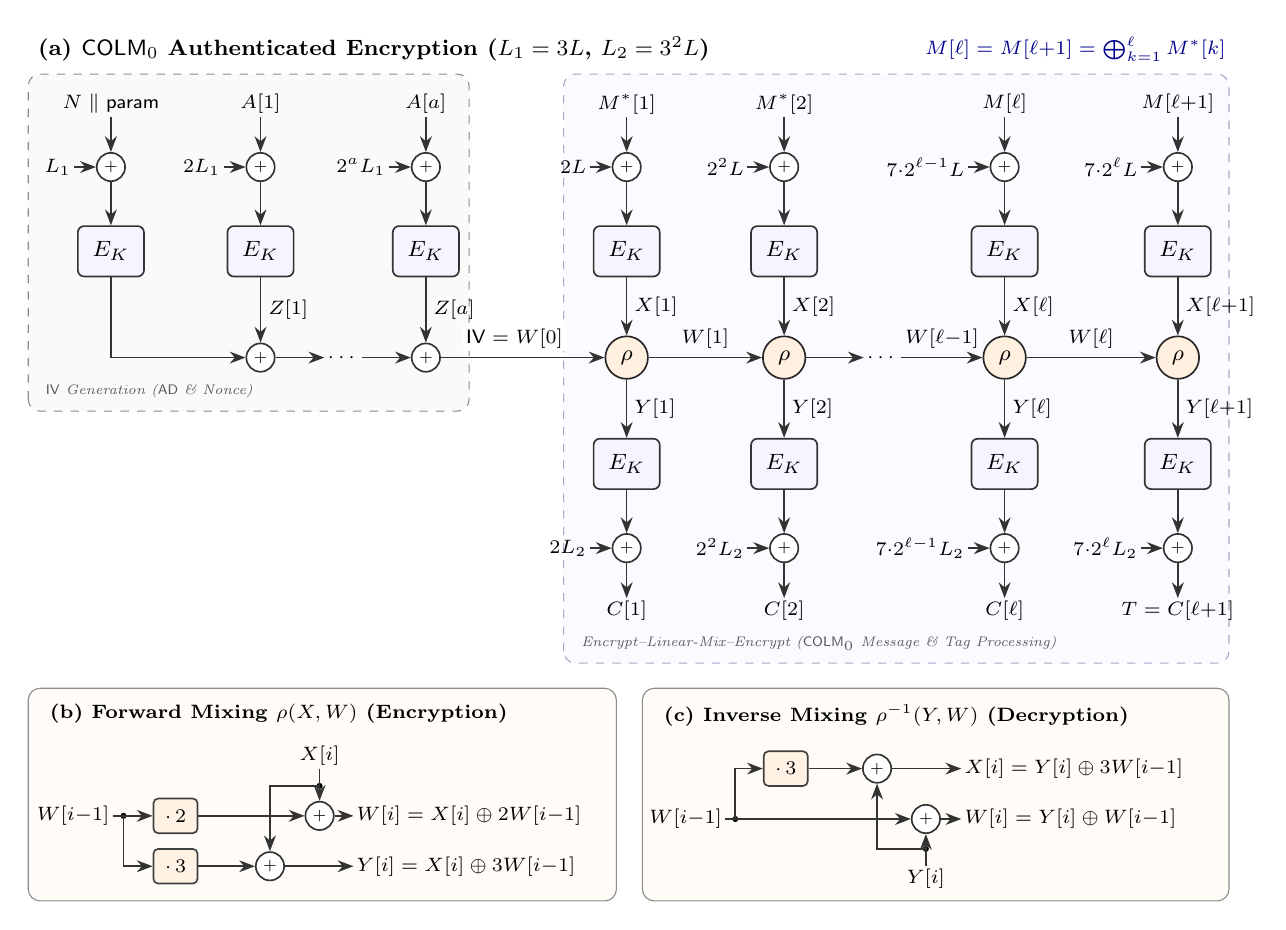
\begin{tikzpicture}[
    >=Stealth,
    bc/.style={rectangle, draw=black!80, semithick, rounded corners=0.8mm, fill=blue!4, minimum width=8.4mm, minimum height=6.4mm, inner sep=1pt, font=\footnotesize\bfseries},
    xor/.style={circle, draw=black!80, semithick, fill=white, minimum size=3.6mm, inner sep=0pt, font=\tiny},
    rhonode/.style={circle, draw=black!85, semithick, fill=orange!12, minimum size=5.4mm, inner sep=0pt, font=\footnotesize},
    mult/.style={rectangle, draw=black!75, semithick, rounded corners=0.6mm, fill=orange!10, minimum width=5.6mm, minimum height=4.4mm, inner sep=1pt, font=\scriptsize},
    lbl/.style={font=\scriptsize, inner sep=1pt},
    wire/.style={->, semithick, draw=black!80},
    lineonly/.style={semithick, draw=black!80}
]

% ================= PANEL (a): OVERALL COLM_0 ARCHITECTURE =================
\node[font=\footnotesize\bfseries, anchor=west] at (-0.15, 3.92) {(a) $\COLMzero$ Authenticated Encryption ($L_1 = 3L$, $L_2 = 3^2 L$)};
\node[lbl, text=blue!55!black, anchor=east] at (15.10, 3.92) {$M[\ell] = M[\ell{+}1] = \bigoplus_{k=1}^{\ell} M^*[k]$};

% Background group boxes
\begin{scope}[on background layer]
    \draw[rounded corners=1.5mm, dashed, draw=black!45, fill=gray!4] (-0.15, -0.68) rectangle (5.45, 3.60);
    \node[font=\tiny\itshape, text=black!65, anchor=south west] at (-0.05, -0.64) {$\IV$ Generation ($\AD$ \& Nonce)};
    \draw[rounded corners=1.5mm, dashed, draw=blue!40!black!35, fill=blue!2] (6.65, -3.88) rectangle (15.10, 3.60);
    \node[font=\tiny\itshape, text=black!65, anchor=south west] at (6.75, -3.84) {Encrypt--Linear-Mix--Encrypt ($\COLMzero$ Message \& Tag Processing)};
\end{scope}

% --- AD Column 0: N || param (x = 0.90) ---
\node[lbl] (ad0) at (0.90, 3.22) {$N \parallel \mathsf{param}$};
\node[xor] (ax0) at (0.90, 2.42) {$+$};
\node[lbl, anchor=east] (am0) at (0.43, 2.42) {$L_1$};
\node[bc]  (ae0) at (0.90, 1.35) {$E_K$};
\draw[wire] (ad0) -- (ax0);
\draw[wire] (am0) -- (ax0);
\draw[wire] (ax0) -- (ae0);

% --- AD Column 1: A[1] (x = 2.80) ---
\node[lbl] (ad1) at (2.80, 3.22) {$A[1]$};
\node[xor] (ax1) at (2.80, 2.42) {$+$};
\node[lbl, anchor=east] (am1) at (2.33, 2.42) {$2 L_1$};
\node[bc]  (ae1) at (2.80, 1.35) {$E_K$};
\node[xor] (aw1) at (2.80, 0.00) {$+$};
\draw[wire] (ad1) -- (ax1);
\draw[wire] (am1) -- (ax1);
\draw[wire] (ax1) -- (ae1);
\draw[wire] (ae1) -- node[lbl, right=1.5pt] {$Z[1]$} (aw1);
\draw[wire] (ae0.south) |- (aw1.west);

% --- AD Dots & Column a: A[a] (x = 4.90) ---
\node[lbl] (addots) at (3.85, 0.00) {$\cdots$};
\draw[wire] (aw1) -- (addots);

\node[lbl] (ada) at (4.90, 3.22) {$A[a]$};
\node[xor] (axa) at (4.90, 2.42) {$+$};
\node[lbl, anchor=east] (ama) at (4.43, 2.42) {$2^a L_1$};
\node[bc]  (aea) at (4.90, 1.35) {$E_K$};
\node[xor] (awa) at (4.90, 0.00) {$+$};
\draw[wire] (ada) -- (axa);
\draw[wire] (ama) -- (axa);
\draw[wire] (axa) -- (aea);
\draw[wire] (aea) -- node[lbl, right=1.5pt] {$Z[a]$} (awa);
\draw[wire] (addots) -- (awa);

% --- Message Column 1: M*[1] (x = 7.45) ---
\node[lbl] (m1)  at (7.45, 3.22) {$M^*[1]$};
\node[xor] (mx1) at (7.45, 2.42) {$+$};
\node[lbl, anchor=east] (mm1) at (6.98, 2.42) {$2L$};
\node[bc]  (ue1) at (7.45, 1.35) {$E_K$};
\node[rhonode] (r1) at (7.45, 0.00) {$\rho$};
\node[bc]  (le1) at (7.45, -1.35) {$E_K$};
\node[xor] (cx1) at (7.45, -2.42) {$+$};
\node[lbl, anchor=east] (cm1) at (6.98, -2.42) {$2 L_2$};
\node[lbl] (c1)  at (7.45, -3.22) {$C[1]$};

\draw[wire] (awa) -- node[lbl, above=2pt, pos=0.45, fill=white, inner sep=1pt] {$\IV = W[0]$} (r1);
\draw[wire] (m1) -- (mx1);
\draw[wire] (mm1) -- (mx1);
\draw[wire] (mx1) -- (ue1);
\draw[wire] (ue1) -- node[lbl, right=1.5pt] {$X[1]$} (r1);
\draw[wire] (r1)  -- node[lbl, right=1.5pt] {$Y[1]$} (le1);
\draw[wire] (le1) -- (cx1);
\draw[wire] (cm1) -- (cx1);
\draw[wire] (cx1) -- (c1);

% --- Message Column 2: M*[2] (x = 9.45) ---
\node[lbl] (m2)  at (9.45, 3.22) {$M^*[2]$};
\node[xor] (mx2) at (9.45, 2.42) {$+$};
\node[lbl, anchor=east] (mm2) at (8.98, 2.42) {$2^2 L$};
\node[bc]  (ue2) at (9.45, 1.35) {$E_K$};
\node[rhonode] (r2) at (9.45, 0.00) {$\rho$};
\node[bc]  (le2) at (9.45, -1.35) {$E_K$};
\node[xor] (cx2) at (9.45, -2.42) {$+$};
\node[lbl, anchor=east] (cm2) at (8.98, -2.42) {$2^2 L_2$};
\node[lbl] (c2)  at (9.45, -3.22) {$C[2]$};

\draw[wire] (r1) -- node[lbl, above=2pt] {$W[1]$} (r2);
\draw[wire] (m2) -- (mx2);
\draw[wire] (mm2) -- (mx2);
\draw[wire] (mx2) -- (ue2);
\draw[wire] (ue2) -- node[lbl, right=1.5pt] {$X[2]$} (r2);
\draw[wire] (r2)  -- node[lbl, right=1.5pt] {$Y[2]$} (le2);
\draw[wire] (le2) -- (cx2);
\draw[wire] (cm2) -- (cx2);
\draw[wire] (cx2) -- (c2);

% --- Message Dots (x = 10.75) ---
\node[lbl] (mdots) at (10.70, 0.00) {$\cdots$};
\draw[wire] (r2) -- (mdots);

% --- Message Column l: M[l] checksum (x = 12.25) ---
\node[lbl] (ml)  at (12.25, 3.22) {$M[\ell]$};
\node[xor] (mxl) at (12.25, 2.42) {$+$};
\node[lbl, anchor=east] (mml) at (11.78, 2.42) {$7{\cdot}2^{\ell-1}L$};
\node[bc]  (uel) at (12.25, 1.35) {$E_K$};
\node[rhonode] (rl) at (12.25, 0.00) {$\rho$};
\node[bc]  (lel) at (12.25, -1.35) {$E_K$};
\node[xor] (cxl) at (12.25, -2.42) {$+$};
\node[lbl, anchor=east] (cml) at (11.78, -2.42) {$7{\cdot}2^{\ell-1}L_2$};
\node[lbl] (cl)  at (12.25, -3.22) {$C[\ell]$};

\draw[wire] (mdots) -- node[lbl, above=2pt] {$W[\ell{-}1]$} (rl);
\draw[wire] (ml) -- (mxl);
\draw[wire] (mml) -- (mxl);
\draw[wire] (mxl) -- (uel);
\draw[wire] (uel) -- node[lbl, right=1.5pt] {$X[\ell]$} (rl);
\draw[wire] (rl)  -- node[lbl, right=1.5pt] {$Y[\ell]$} (lel);
\draw[wire] (lel) -- (cxl);
\draw[wire] (cml) -- (cxl);
\draw[wire] (cxl) -- (cl);

% --- Tag Column l+1: M[l+1] = M[l] (x = 14.45) ---
\node[lbl] (mt)  at (14.45, 3.22) {$M[\ell{+}1]$};
\node[xor] (mxt) at (14.45, 2.42) {$+$};
\node[lbl, anchor=east] (mmt) at (13.98, 2.42) {$7{\cdot}2^{\ell}L$};
\node[bc]  (uet) at (14.45, 1.35) {$E_K$};
\node[rhonode] (rt) at (14.45, 0.00) {$\rho$};
\node[bc]  (let) at (14.45, -1.35) {$E_K$};
\node[xor] (cxt) at (14.45, -2.42) {$+$};
\node[lbl, anchor=east] (cmt) at (13.98, -2.42) {$7{\cdot}2^{\ell}L_2$};
\node[lbl] (ct)  at (14.45, -3.22) {$T = C[\ell{+}1]$};

\draw[wire] (rl) -- node[lbl, above=2pt] {$W[\ell]$} (rt);
\draw[wire] (mt) -- (mxt);
\draw[wire] (mmt) -- (mxt);
\draw[wire] (mxt) -- (uet);
\draw[wire] (uet) -- node[lbl, right=1.5pt] {$X[\ell{+}1]$} (rt);
\draw[wire] (rt)  -- node[lbl, right=1.5pt] {$Y[\ell{+}1]$} (let);
\draw[wire] (let) -- (cxt);
\draw[wire] (cmt) -- (cxt);
\draw[wire] (cxt) -- (ct);

% ================= PANEL (b) & (c): LINEAR MIXING CIRCUITS =================
% --- Panel (b): Forward rho (Encryption) ---
\begin{scope}[yshift=-5.78cm, xshift=0.0cm]
    \draw[rounded corners=1.5mm, draw=black!45, fill=orange!3] (-0.15, -1.12) rectangle (7.32, 1.58);
    \node[font=\scriptsize\bfseries, anchor=north west] at (0.0, 1.50) {(b) Forward Mixing $\rho(X, W)$ (Encryption)};

    \node[lbl] (b_win) at (0.42, -0.04) {$W[i{-}1]$};
    \node[lbl] (b_xin) at (3.55, 0.72) {$X[i]$};
    \node[mult] (b_m2) at (1.72, -0.04) {$\cdot\, 2$};
    \node[mult] (b_m3) at (1.72, -0.68) {$\cdot\, 3$};
    \node[xor]  (b_xw) at (3.55, -0.04) {$+$};
    \node[xor]  (b_xy) at (2.92, -0.68) {$+$};
    \node[lbl, anchor=west] (b_wout) at (3.98, -0.04) {$W[i] = X[i] \oplus 2W[i{-}1]$};
    \node[lbl, anchor=west] (b_yout) at (3.98, -0.68) {$Y[i] = X[i] \oplus 3W[i{-}1]$};

    \coordinate (b_splitw) at (1.06, -0.04);
    \coordinate (b_splitx) at (3.55, 0.34);
    \fill (b_splitw) circle (1.1pt);
    \fill (b_splitx) circle (1.1pt);

    \draw[wire] (b_win) -- (b_m2);
    \draw[wire] (b_splitw) |- (b_m3);
    \draw[wire] (b_m2) -- (b_xw);
    \draw[wire] (b_m3) -- (b_xy);
    \draw[lineonly] (b_xin) -- (b_splitx);
    \draw[wire] (b_splitx) -- (b_xw);
    \draw[wire] (b_splitx) -| (b_xy);
    \draw[wire] (b_xw) -- (b_wout);
    \draw[wire] (b_xy) -- (b_yout);
\end{scope}

% --- Panel (c): Inverse rho^{-1} (Decryption) ---
\begin{scope}[yshift=-5.78cm, xshift=7.65cm]
    \draw[rounded corners=1.5mm, draw=black!45, fill=orange!3] (0.0, -1.12) rectangle (7.45, 1.58);
    \node[font=\scriptsize\bfseries, anchor=north west] at (0.15, 1.50) {(c) Inverse Mixing $\rho^{-1}(Y, W)$ (Decryption)};

    \node[lbl] (c_win) at (0.55, -0.08) {$W[i{-}1]$};
    \node[lbl] (c_yin) at (3.60, -0.84) {$Y[i]$};
    \node[mult] (c_m3) at (1.82, 0.56) {$\cdot\, 3$};
    \node[xor]  (c_xx) at (2.98, 0.56) {$+$};
    \node[xor]  (c_xw) at (3.60, -0.08) {$+$};
    \node[lbl, anchor=west] (c_xout) at (4.05, 0.56) {$X[i] = Y[i] \oplus 3W[i{-}1]$};
    \node[lbl, anchor=west] (c_wout) at (4.05, -0.08) {$W[i] = Y[i] \oplus W[i{-}1]$};

    \coordinate (c_splitw) at (1.18, -0.08);
    \coordinate (c_splity) at (3.60, -0.46);
    \fill (c_splitw) circle (1.1pt);
    \fill (c_splity) circle (1.1pt);

    \draw[wire] (c_win) -- (c_xw);
    \draw[wire] (c_splitw) |- (c_m3);
    \draw[wire] (c_m3) -- (c_xx);
    \draw[lineonly] (c_yin) -- (c_splity);
    \draw[wire] (c_splity) -- (c_xw);
    \draw[wire] (c_splity) -| (c_xx);
    \draw[wire] (c_xx) -- (c_xout);
    \draw[wire] (c_xw) -- (c_wout);
\end{scope}

\end{tikzpicture}
\caption{Overall Encrypt--Linear-Mix--Encrypt architecture of $\COLMzero$ (adapted from~\cite[Figure~1.1]{COLMv1} and~\cite[Figure~1]{COLM24}). \textbf{(a)}~Parallel $\AD$/nonce initialization produces the initial chaining state $\IV = W[0]$; each message/tag column $i$ then traverses an upper blockcipher layer ($E_K$), a stateful linear mixing layer ($\rho$) threaded horizontally by $W[0] \to W[1] \to \dots \to W[\ell]$, and a lower blockcipher layer ($E_K$). \textbf{(b)}~Forward linear mixing $\rho$ in encryption. \textbf{(c)}~Inverse linear mixing $\rho^{-1}$ in decryption, where the chaining update simplifies to $W[i] = W[i-1] \oplus Y[i]$.}
\label{fig:colm-arch}
\end{figure}

As illustrated in Figure~\ref{fig:colm-arch}(a) (adapted from~\cite[Figure~1.1, p.~4]{COLMv1} and~\cite[Figure~1, p.~10]{COLM24}), $\COLMzero$ processes every query in two sequential stages:
\begin{enumerate}[leftmargin=2em]
    \item \textbf{Stage~1 --- Parallel Nonce and Associated-Data Initialization ($\IV$ Generation):} In the left dashed box of Figure~\ref{fig:colm-arch}(a), the $64$-bit nonce $N$ is concatenated with the $64$-bit parameter descriptor $\mathsf{param}$ ($0^{64}$ in $\COLMzero$) to form an initial header block $A[0] = N \parallel \mathsf{param}$. A PMAC-style parallel layer masks $A[0]$ and each associated-data block $A[1], \dots, A[a]$ with distinct subkey masks $\Delta_A[0 \dots a]$, encrypts each masked block independently under $E_K$, and XORs all $a + 1$ outputs to form a $128$-bit initial value $\IV$. This $\IV$ initializes the horizontal chaining register entering the message pipeline: $W[0] \leftarrow \IV$.
    \item \textbf{Stage~2 --- Encrypt--Linear-Mix--Encrypt ($\mathsf{ELE}$) Message and Tag Pipeline:} Prior to encryption, $\COLMzero$ maps the $\ell$ plaintext blocks $M^*[1 \dots \ell]$ into $\ell + 1$ internal $128$-bit input blocks. It retains $M[i] = M^*[i]$ for $1 \le i \le \ell - 1$, replaces the $\ell$-th block with the full plaintext XOR checksum $M[\ell] = \bigoplus_{k=1}^\ell M^*[k]$, and appends a duplicate checksum block $M[\ell+1] = M[\ell]$ dedicated to tag generation. In the right dashed box of Figure~\ref{fig:colm-arch}(a), each column $i \in \{1, \dots, \ell+1\}$ passes top-to-bottom through two keyed blockcipher layers separated by a stateful linear mixing layer. Meanwhile, a $128$-bit \emph{chaining state} $W[0] \to W[1] \to \dots \to W[\ell]$ propagates horizontally from left to right:
    \begin{itemize}[leftmargin=1.5em]
        \item \emph{Upper blockcipher layer:} This layer comprises the top row of $E_K$ invocations on the message path. At column~$i$, the internal block $M[i]$ is masked with an XEX plaintext mask $\Delta_M[i]$ and encrypted via $E_K$ to produce the \emph{upper-layer output} $X[i] = E_K(M[i] \oplus \Delta_M[i])$. Notice that this layer operates strictly block-by-block in parallel and receives no input from $(N, A)$ or earlier blocks.
        \item \emph{Middle linear mixing layer ($\rho$) and chaining state ($W$):} Positioned between the two blockcipher rows, the invertible linear map $\rho$ couples column~$i$'s upper-layer output $X[i]$ with the \emph{incoming chaining state} $W[i-1]$. That state is the $128$-bit horizontal state register emitted by the preceding column $i - 1$, initialized at $i = 1$ to $W[0] = \IV$. Evaluating $(Y[i], W[i]) = \rho(X[i], W[i-1])$ simultaneously computes the mixed vertical block $Y[i]$ fed into column~$i$'s second blockcipher call and the \emph{updated chaining state} $W[i]$ passed horizontally as the incoming state to column~$i + 1$. This horizontal state wire is the sole mechanism diffusing the $(N, A)$-dependent $\IV$ and prior message blocks $M[1 \dots i-1]$ into subsequent ciphertext blocks and the tag.
        \item \emph{Lower blockcipher layer:} This layer comprises the bottom row of $E_K$ invocations on the message path. At column~$i$, the mixed state $Y[i]$ is encrypted through a second $E_K$ call and XORed with a ciphertext mask $\Delta_C[i]$ to output $C[i] = E_K(Y[i]) \oplus \Delta_C[i]$. This produces ciphertext blocks for $1 \le i \le \ell$ and the authentication tag $T = C[\ell+1]$ at $i = \ell+1$.
    \end{itemize}
\end{enumerate}
\paragraph{Inverse Dataflow During Decryption.}
When decrypting $C[1 \dots \ell+1]$ under $(N, A)$, the receiver first recomputes the identical initial chaining state $W[0] = \IV$ via Stage~1. It then traverses columns $i = 1, \dots, \ell$ from bottom to top. At each column it inverts the \emph{lower blockcipher layer} via $Y[i] = E_K^{-1}(C[i] \oplus \Delta_C[i])$. It next combines $Y[i]$ with the \emph{incoming chaining state} $W[i-1]$ through the \emph{inverse linear mixing map} $(X[i], W[i]) = \rho^{-1}(Y[i], W[i-1])$ (Figure~\ref{fig:colm-arch}(c)) to recover the upper-layer state $X[i]$ while advancing the chaining state to $W[i]$. Finally it inverts the \emph{upper blockcipher layer} via $\tilde{M}[i] = E_K^{-1}(X[i]) \oplus \Delta_M[i]$. At column $\ell+1$, the receiver evaluates a forward tag-verification pass from the recovered checksum and $W[\ell]$ to test whether $\tilde{C}[\ell+1] = C[\ell+1]$.

\subsection{Field Arithmetic, Masking Schedule, and Linear Mixing}
With the architectural dataflow established, we state the algebraic definitions of the field arithmetic, the XEX masks, and the mixing maps $\rho$ and $\rho^{-1}$. Every $128$-bit block ($n = 128$) is identified with an element of the binary extension field
\begin{equation}
\label{eq:field}
\FtwoN = \Ftwo[x] / \big(f(x)\big), \qquad f(x) = x^{128} + x^7 + x^2 + x + 1.
\end{equation}
In the integer notation of~\cite[Section~1.1, pp.~1--2]{COLMv1}, the field element $x \in \FtwoN$ is written as $2$, $x + 1$ is written as $3$, and $x^2 + x + 1 = 3^2 \oplus 2$ is written as $7$. Throughout this paper, addition in $\FtwoN$ is bitwise XOR ($\oplus$), and juxtaposition or $(\cdot)$ denotes multiplication in $\FtwoN$ modulo $f(x)$.

\paragraph{Subkey and Masking Schedule ($\Delta_A, \Delta_M, \Delta_C$).}
From the secret key $K$, $\COLM$ derives a single secret mask base $L \leftarrow E_K(0^{128}) \in \FtwoN$. It then initializes three domain-separated base masks~\cite[Section~1.4, pp.~4--5]{COLMv1}, \cite[Figures~2--3, pp.~11--12]{COLM24}, one each for Stage~1 header hashing, the upper blockcipher layer, and the lower blockcipher layer:
\begin{equation}
\label{eq:base-masks}
\Delta_0 \leftarrow 3 \cdot 2^{-1} L, \qquad \Delta_1 \leftarrow L, \qquad \Delta_2 \leftarrow 3^2 L.
\end{equation}
On the header block $A[0] = N \parallel \mathsf{param}$, Stage~1 uses $\Delta_A[0] = 2\Delta_0 = 3L$; for non-empty associated data ($a = \lceil |A|/128 \rceil \ge 1$), the $\AD$ mask multiplies by $2$ (i.e., $x$) on every non-final block ($1 \le j < a$) and on a complete final block ($|A| = 128a$), and by $7$ on an incomplete ($10^*$-padded) final block ($|A| < 128a$). In Stage~2, the message and ciphertext masks ($\Delta_M, \Delta_C$) multiply by $2$ on every non-final message block ($1 \le i \le \ell - 1$), by $7$ on a complete final message block ($i = \ell$), by $7^2$ on an incomplete ($10^*$-padded) final message block ($i = \ell$), and by $2$ again on the tag block ($i = \ell + 1$). Thus, for a message of $\ell$ complete $128$-bit blocks, the upper-layer plaintext masks $\Delta_M[i]$ and lower-layer ciphertext masks $\Delta_C[i]$ are:
\begin{equation}
\label{eq:masks}
\Delta_M[i] = \begin{cases}
2^i L & \text{for } 1 \le i \le \ell - 1, \\
7 \cdot 2^{\ell-1} L & \text{for } i = \ell, \\
7 \cdot 2^\ell L & \text{for } i = \ell + 1 \text{ (tag block)},
\end{cases}
\qquad
\Delta_C[i] = 3^2 \, \Delta_M[i] \quad (1 \le i \le \ell + 1).
\end{equation}
By~\eqref{eq:masks}, \emph{$\Delta_M[i]$ and $\Delta_C[i]$ depend solely on the secret key $K$ (via $L$), the block index $i$, and the message length $\ell$. They depend neither on the nonce $N$ nor on the associated data $A$}.

\paragraph{The Linear Mixing Map $\rho$ and Its Inverse $\rho^{-1}$.}
At column $i$ of Stage~2, let $X[i] \in \FtwoN$ be the output of the upper blockcipher layer and $W[i-1] \in \FtwoN$ the incoming horizontal chaining state from column $i-1$ (with $W[0] = \IV$). Let $Y[i] \in \FtwoN$ be the input to the lower blockcipher layer and $W[i] \in \FtwoN$ the updated horizontal chaining state passed to column $i+1$. As depicted in Figures~\ref{fig:colm-arch}(b) and~\ref{fig:colm-arch}(c), the forward mixing map $\rho(X, W) = (Y, W')$ and the inverse mixing map $\rho^{-1}(Y, W) = (X, W')$~\cite[Section~1.3, p.~3]{COLMv1} used during encryption and decryption, respectively, are defined over $\FtwoN$ by:
\begin{equation}
\label{eq:rho}
\rho(X, W) = \begin{pmatrix} Y \\ W' \end{pmatrix} = \begin{pmatrix} 1 & 3 \\ 1 & 2 \end{pmatrix} \begin{pmatrix} X \\ W \end{pmatrix} = \begin{pmatrix} X \oplus 3W \\ X \oplus 2W \end{pmatrix},
\end{equation}
where $3 \oplus 2 = (x + 1) \oplus x = 1$ holds in $\FtwoN$. Substituting $X = Y \oplus 3W$ into $W' = X \oplus 2W$ therefore cancels the multiplier on $W$, giving
\begin{equation}
\label{eq:rho-inv}
\rho^{-1}(Y, W) = \begin{pmatrix} X \\ W' \end{pmatrix} = \begin{pmatrix} 1 & 3 \\ 1 & 1 \end{pmatrix} \begin{pmatrix} Y \\ W \end{pmatrix} = \begin{pmatrix} Y \oplus 3W \\ Y \oplus W \end{pmatrix}.
\end{equation}
Whereas encryption advances the chaining state via field multiplication by $2$ ($W[i] = X[i] \oplus 2W[i-1]$), decryption~\eqref{eq:rho-inv} reduces the horizontal chaining update to the plain running XOR of the lower-layer intermediate states:
\begin{equation}
\label{eq:W-running-xor}
W[i] = W[i-1] \oplus Y[i] = \IV \oplus \bigoplus_{j=1}^{i} Y[j] \qquad \forall i \ge 1.
\end{equation}

\subsection{Complete Algorithmic Flow of \texorpdfstring{$\COLMzero$}{COLM\_0}}
To complement the encryption diagram in Figure~\ref{fig:colm-arch}(a), Figure~\ref{fig:colm-dec} illustrates the verified decryption and tag-checking architecture $\mathsf{COLM}_0\text{-}\mathsf{Dec}_K(N, A, C[1 \dots \ell+1])$. Algorithm~1 gives the joint pseudocode of both procedures~\cite[Sections~1.4--1.5, pp.~4--8]{COLMv1}. In Figure~\ref{fig:colm-dec}, Stage~1 recomputes $\IV = W[0]$ in the forward direction ($E_K$). Message columns $i = 1, \dots, \ell$ run bottom-to-top through $E_K^{-1}$ and $\rho^{-1}$ while advancing $W[i] = W[i-1] \oplus Y[i]$ horizontally. Following~\cite[Section~1.5.3, p.~8]{COLMv1} and~\cite[Figure~3, p.~12]{COLM24}, column $\ell+1$ then runs top-to-bottom from $\CS$ and $W[\ell]$ via $E_K$ and $\rho$ to recompute $\tilde{C}[\ell+1]$ and test $\tilde{C}[\ell+1] \stackrel{?}{=} C[\ell+1]$ before releasing $\tilde{M}^*[1 \dots \ell]$ or returning $\perp$.

\begin{figure}[t!]
\centering
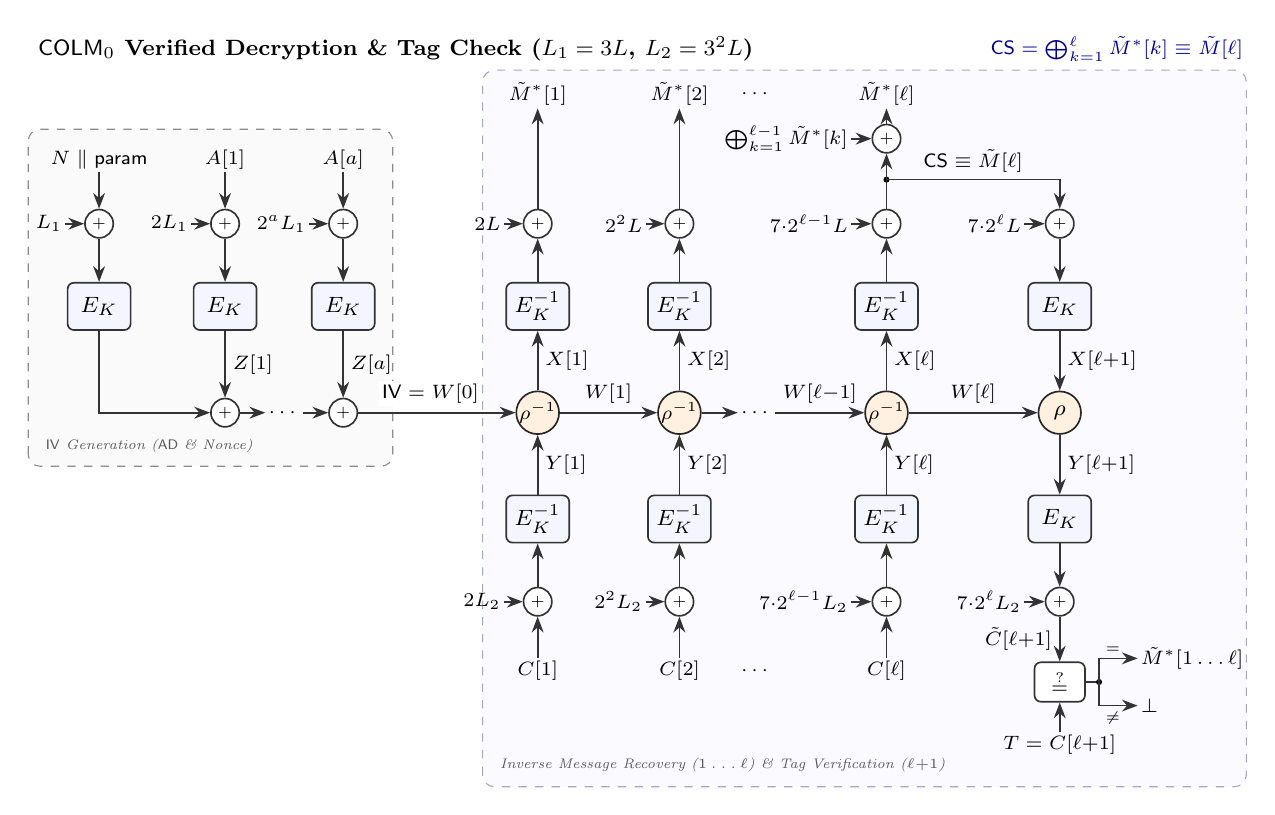
\begin{tikzpicture}[
    >=Stealth,
    bc/.style={rectangle, draw=black!80, semithick, rounded corners=0.8mm, fill=blue!4, minimum width=8.0mm, minimum height=6.0mm, inner sep=1pt, font=\footnotesize\bfseries},
    bcinv/.style={rectangle, draw=black!80, semithick, rounded corners=0.8mm, fill=blue!4, minimum width=8.0mm, minimum height=6.0mm, inner sep=1pt, font=\footnotesize\bfseries},
    xor/.style={circle, draw=black!80, semithick, fill=white, minimum size=3.6mm, inner sep=0pt, font=\tiny},
    rhonode/.style={circle, draw=black!85, semithick, fill=orange!12, minimum size=5.4mm, inner sep=0pt, font=\footnotesize},
    rhoinv/.style={circle, draw=black!85, semithick, fill=orange!12, minimum size=5.4mm, inner sep=0pt, font=\scriptsize},
    cmpnode/.style={rectangle, draw=black!80, semithick, rounded corners=0.8mm, fill=white, minimum width=6.4mm, minimum height=5.0mm, inner sep=1pt, font=\scriptsize\bfseries},
    lbl/.style={font=\scriptsize, inner sep=1pt},
    wire/.style={->, semithick, draw=black!80},
    lineonly/.style={semithick, draw=black!80}
]

% Header banner
\node[font=\footnotesize\bfseries, anchor=west] at (-0.15, 4.62) {$\COLMzero$ Verified Decryption \& Tag Check ($L_1 = 3L$, $L_2 = 3^2 L$)};
\node[lbl, text=blue!55!black, anchor=east] at (15.32, 4.62) {$\CS = \bigoplus_{k=1}^{\ell} \tilde{M}^*[k] \equiv \tilde{M}[\ell]$};

% Background group boxes
\begin{scope}[on background layer]
    \draw[rounded corners=1.5mm, dashed, draw=black!45, fill=gray!4] (-0.15, -0.68) rectangle (4.48, 3.60);
    \node[font=\tiny\itshape, text=black!65, anchor=south west] at (-0.05, -0.64) {$\IV$ Generation ($\AD$ \& Nonce)};
    \draw[rounded corners=1.5mm, dashed, draw=blue!40!black!35, fill=blue!2] (5.62, -4.75) rectangle (15.32, 4.35);
    \node[font=\tiny\itshape, text=black!65, anchor=south west] at (5.72, -4.69) {Inverse Message Recovery ($1 \dots \ell$) \& Tag Verification ($\ell{+}1$)};
\end{scope}

% --- Stage 1 AD Column 0: N || param (x = 0.75) ---
\node[lbl] (ad0) at (0.75, 3.22) {$N \parallel \mathsf{param}$};
\node[xor] (ax0) at (0.75, 2.40) {$+$};
\node[lbl, anchor=east] (am0) at (0.32, 2.40) {$L_1$};
\node[bc]  (ae0) at (0.75, 1.35) {$E_K$};
\draw[wire] (ad0) -- (ax0);
\draw[wire] (am0) -- (ax0);
\draw[wire] (ax0) -- (ae0);

% --- Stage 1 AD Column 1: A[1] (x = 2.35) ---
\node[lbl] (ad1) at (2.35, 3.22) {$A[1]$};
\node[xor] (ax1) at (2.35, 2.40) {$+$};
\node[lbl, anchor=east] (am1) at (1.92, 2.40) {$2 L_1$};
\node[bc]  (ae1) at (2.35, 1.35) {$E_K$};
\node[xor] (aw1) at (2.35, 0.00) {$+$};
\draw[wire] (ad1) -- (ax1);
\draw[wire] (am1) -- (ax1);
\draw[wire] (ax1) -- (ae1);
\draw[wire] (ae1) -- node[lbl, right=1.5pt] {$Z[1]$} (aw1);
\draw[wire] (ae0.south) |- (aw1.west);

% --- Stage 1 AD Dots & Column a: A[a] (x = 3.85) ---
\node[lbl] (addots) at (3.10, 0.00) {$\cdots$};
\draw[wire] (aw1) -- (addots);

\node[lbl] (ada) at (3.85, 3.22) {$A[a]$};
\node[xor] (axa) at (3.85, 2.40) {$+$};
\node[lbl, anchor=east] (ama) at (3.42, 2.40) {$2^a L_1$};
\node[bc]  (aea) at (3.85, 1.35) {$E_K$};
\node[xor] (awa) at (3.85, 0.00) {$+$};
\draw[wire] (ada) -- (axa);
\draw[wire] (ama) -- (axa);
\draw[wire] (axa) -- (aea);
\draw[wire] (aea) -- node[lbl, right=1.5pt] {$Z[a]$} (awa);
\draw[wire] (addots) -- (awa);

% --- Decryption Column 1: C[1] -> M~*[1] (x = 6.32) ---
\node[lbl]   (c1)  at (6.32, -3.28) {$C[1]$};
\node[xor]   (cx1) at (6.32, -2.40) {$+$};
\node[lbl, anchor=east] (cm1) at (5.89, -2.40) {$2 L_2$};
\node[bcinv] (le1) at (6.32, -1.35) {$E_K^{-1}$};
\node[rhoinv](r1)  at (6.32,  0.00) {$\rho^{-1}$};
\node[bcinv] (ue1) at (6.32,  1.35) {$E_K^{-1}$};
\node[xor]   (mx1) at (6.32,  2.40) {$+$};
\node[lbl, anchor=east] (mm1) at (5.89,  2.40) {$2 L$};
\node[lbl]   (m1)  at (6.32,  4.05) {$\tilde{M}^*[1]$};

\draw[wire] (awa) -- node[lbl, above=2pt, pos=0.46, fill=white, inner sep=1pt] {$\IV = W[0]$} (r1);
\draw[wire] (c1)  -- (cx1);
\draw[wire] (cm1) -- (cx1);
\draw[wire] (cx1) -- (le1);
\draw[wire] (le1) -- node[lbl, right=1.5pt] {$Y[1]$} (r1);
\draw[wire] (r1)  -- node[lbl, right=1.5pt] {$X[1]$} (ue1);
\draw[wire] (ue1) -- (mx1);
\draw[wire] (mm1) -- (mx1);
\draw[wire] (mx1) -- (m1);

% --- Decryption Column 2: C[2] -> M~*[2] (x = 8.12) ---
\node[lbl]   (c2)  at (8.12, -3.28) {$C[2]$};
\node[xor]   (cx2) at (8.12, -2.40) {$+$};
\node[lbl, anchor=east] (cm2) at (7.69, -2.40) {$2^2 L_2$};
\node[bcinv] (le2) at (8.12, -1.35) {$E_K^{-1}$};
\node[rhoinv](r2)  at (8.12,  0.00) {$\rho^{-1}$};
\node[bcinv] (ue2) at (8.12,  1.35) {$E_K^{-1}$};
\node[xor]   (mx2) at (8.12,  2.40) {$+$};
\node[lbl, anchor=east] (mm2) at (7.69,  2.40) {$2^2 L$};
\node[lbl]   (m2)  at (8.12,  4.05) {$\tilde{M}^*[2]$};

\draw[wire] (r1)  -- node[lbl, above=2pt] {$W[1]$} (r2);
\draw[wire] (c2)  -- (cx2);
\draw[wire] (cm2) -- (cx2);
\draw[wire] (cx2) -- (le2);
\draw[wire] (le2) -- node[lbl, right=1.5pt] {$Y[2]$} (r2);
\draw[wire] (r2)  -- node[lbl, right=1.5pt] {$X[2]$} (ue2);
\draw[wire] (ue2) -- (mx2);
\draw[wire] (mm2) -- (mx2);
\draw[wire] (mx2) -- (m2);

% --- Dots (x = 9.10) ---
\node[lbl] (mdots) at (9.10,  0.00) {$\cdots$};
\node[lbl] (tdots) at (9.10,  4.05) {$\cdots$};
\node[lbl] (bdots) at (9.10, -3.28) {$\cdots$};
\draw[wire] (r2) -- (mdots);

% --- Decryption Column l: C[l] -> M~[l] -> M~*[l] & CS (x = 10.75) ---
\node[lbl]   (cl)  at (10.75, -3.28) {$C[\ell]$};
\node[xor]   (cxl) at (10.75, -2.40) {$+$};
\node[lbl, anchor=east] (cml) at (10.30, -2.40) {$7{\cdot}2^{\ell-1}L_2$};
\node[bcinv] (lel) at (10.75, -1.35) {$E_K^{-1}$};
\node[rhoinv](rl)  at (10.75,  0.00) {$\rho^{-1}$};
\node[bcinv] (uel) at (10.75,  1.35) {$E_K^{-1}$};
\node[xor]   (mxl) at (10.75,  2.40) {$+$};
\node[lbl, anchor=east] (mml) at (10.30,  2.40) {$7{\cdot}2^{\ell-1}L$};
\coordinate  (msplit) at (10.75, 2.96);
\fill (msplit) circle (1.1pt);
\node[xor]   (csx) at (10.75,  3.48) {$+$};
\node[lbl, anchor=east] (pcs) at (10.30,  3.48) {$\bigoplus_{k=1}^{\ell-1}\tilde{M}^*[k]$};
\node[lbl]   (ml)  at (10.75,  4.05) {$\tilde{M}^*[\ell]$};

\draw[wire]     (mdots) -- node[lbl, above=2pt] {$W[\ell{-}1]$} (rl);
\draw[wire]     (cl)  -- (cxl);
\draw[wire]     (cml) -- (cxl);
\draw[wire]     (cxl) -- (lel);
\draw[wire]     (lel) -- node[lbl, right=1.5pt] {$Y[\ell]$} (rl);
\draw[wire]     (rl)  -- node[lbl, right=1.5pt] {$X[\ell]$} (uel);
\draw[wire]     (uel) -- (mxl);
\draw[wire]     (mml) -- (mxl);
\draw[lineonly] (mxl) -- (msplit);
\draw[wire]     (msplit) -- (csx);
\draw[wire]     (pcs) -- (csx);
\draw[wire]     (csx) -- (ml);

% --- Forward Tag-Check Column l+1: CS -> C~[l+1] == C[l+1] (x = 12.95) ---
\node[xor]     (mxt) at (12.95,  2.40) {$+$};
\node[lbl, anchor=east] (mmt) at (12.50,  2.40) {$7{\cdot}2^{\ell}L$};
\node[bc]      (uet) at (12.95,  1.35) {$E_K$};
\node[rhonode] (rt)  at (12.95,  0.00) {$\rho$};
\node[bc]      (let) at (12.95, -1.35) {$E_K$};
\node[xor]     (cxt) at (12.95, -2.40) {$+$};
\node[lbl, anchor=east] (cmt) at (12.50, -2.40) {$7{\cdot}2^{\ell}L_2$};
\node[cmpnode] (cmp) at (12.95, -3.42) {$\stackrel{?}{=}$};
\node[lbl]     (tin) at (12.95, -4.22) {$T = C[\ell{+}1]$};

\draw[wire] (msplit) -- node[lbl, above=1.5pt] {$\CS \equiv \tilde{M}[\ell]$} (12.95, 2.96) -- (mxt);
\draw[wire] (mmt) -- (mxt);
\draw[wire] (mxt) -- (uet);
\draw[wire] (rl)  -- node[lbl, above=2pt] {$W[\ell]$} (rt);
\draw[wire] (uet) -- node[lbl, right=1.5pt] {$X[\ell{+}1]$} (rt);
\draw[wire] (rt)  -- node[lbl, right=1.5pt] {$Y[\ell{+}1]$} (let);
\draw[wire] (let) -- (cxt);
\draw[wire] (cmt) -- (cxt);
\draw[wire] (cxt) -- node[lbl, left=1.5pt] {$\tilde{C}[\ell{+}1]$} (cmp);
\draw[wire] (tin) -- (cmp);

% --- Verification Decision Output (right of comparator) ---
\coordinate (vsplit) at (13.45, -3.42);
\draw[lineonly] (cmp.east) -- (vsplit);
\fill (vsplit) circle (1.1pt);
\node[lbl, anchor=west] (vacc) at (13.94, -3.12) {$\tilde{M}^*[1 \dots \ell]$};
\node[lbl, anchor=west] (vrej) at (13.94, -3.72) {$\perp$};
\draw[wire] (vsplit) |- node[lbl, above=1pt, pos=0.68] {\tiny $=$} (vacc.west);
\draw[wire] (vsplit) |- node[lbl, below=1pt, pos=0.68] {\tiny $\neq$} (vrej.west);

\end{tikzpicture}
\caption{Complete verified decryption and tag-checking architecture of $\COLMzero$ ($\mathsf{COLM}_0\text{-}\mathsf{Dec}$, mirroring Figure~\ref{fig:colm-arch}(a)). Stage~1 recomputes $\IV = W[0]$ via forward $E_K$ calls; columns $1, \dots, \ell$ invert the lower and upper blockcipher layers ($E_K^{-1}$) and linear mixing ($\rho^{-1}$) bottom-to-top while advancing $W[i] = W[i-1] \oplus Y[i]$. At column~$\ell$, $\tilde{M}[\ell]$ both unmasks the final plaintext block $\tilde{M}^*[\ell]$ and feeds $\CS = \bigoplus_{k=1}^\ell \tilde{M}^*[k] \equiv \tilde{M}[\ell]$ (Lemma~\ref{lem:telescoping}) into the forward tag-verification column $\ell+1$, which releases $\tilde{M}^*[1 \dots \ell]$ if and only if $\tilde{C}[\ell+1] = C[\ell+1]$.}
\label{fig:colm-dec}
\end{figure}

\begin{figure}[t]
\centering
\small
\begin{tabular}{@{}p{0.97\textwidth}@{}}
\toprule
\textbf{Algorithm 1:} $\COLMzero$ Authenticated Encryption ($\mathsf{COLM}_0\text{-}\mathsf{Enc}$) and Verified Decryption ($\mathsf{COLM}_0\text{-}\mathsf{Dec}$) \\
\midrule
\textbf{Shared Key \& AD Initialization $\mathsf{Init}(K, N, A)$:} \\
\hspace*{1.2em} \textbf{1.} $L \leftarrow E_K(0^{128})$; \quad $A[0] \leftarrow N \,\|\, \mathsf{param}$; \quad $a \leftarrow \lceil |A|/128 \rceil$; \quad if $a \ge 1$, parse $A$ into $A[1], \dots, A[a]$ ($10^*$-padded if $|A| < 128a$). \\
\hspace*{1.2em} \textbf{2.} Set $\Delta_A[0] \leftarrow 3L$. If $a \ge 1$, set $\Delta_A[j] \leftarrow 3 \cdot 2^j L$ for $1 \le j < a$, and $\Delta_A[a] \leftarrow 3 \cdot 2^a L$ if $|A| = 128a$ (complete) or $3 \cdot 7 \cdot 2^{a-1} L$ if $|A| < 128a$ (padded). \\
\hspace*{1.2em} \textbf{3.} $\IV = W[0] \leftarrow \bigoplus_{j=0}^{a} E_K\big(A[j] \oplus \Delta_A[j]\big)$. \\[4pt]
\midrule
\textbf{Encryption $\mathsf{COLM}_0\text{-}\mathsf{Enc}_K(N, A, M^*[1 \dots \ell])$:} \hfill (for complete final block $|M^*[\ell]| = 128$) \\
\hspace*{1.2em} \textbf{1.} Run $(L, W[0]) \leftarrow \mathsf{Init}(K, N, A)$ and set the message/tag masks $\Delta_M[1 \dots \ell+1], \Delta_C[1 \dots \ell+1]$ via~\eqref{eq:masks}. \\
\hspace*{1.2em} \textbf{2.} Define the internal message blocks $M[i] \leftarrow M^*[i]$ for $1 \le i \le \ell - 1$, and the checksum block: \\
\hspace*{3.0em} $M[\ell] \leftarrow \bigoplus_{i=1}^{\ell} M^*[i], \qquad M[\ell + 1] \leftarrow M[\ell]$. \\
\hspace*{1.2em} \textbf{3.} \textbf{for} $i = 1$ \textbf{to} $\ell + 1$ \textbf{do} \\
\hspace*{3.0em} $X[i] \leftarrow E_K\big(M[i] \oplus \Delta_M[i]\big)$; \\
\hspace*{3.0em} $Y[i] \leftarrow X[i] \oplus 3W[i-1]$; \quad $W[i] \leftarrow X[i] \oplus 2W[i-1]$; \hfill $\triangleright\; (Y[i], W[i]) = \rho(X[i], W[i-1])$ \\
\hspace*{3.0em} $C[i] \leftarrow E_K(Y[i]) \oplus \Delta_C[i]$; \\
\hspace*{1.2em} \textbf{4.} \textbf{return} ciphertext $C[1 \dots \ell]$ and authentication tag $T = C[\ell + 1]$ (total $\ell + 1$ blocks). \\[4pt]
\midrule
\textbf{Verified Decryption $\mathsf{COLM}_0\text{-}\mathsf{Dec}_K(N, A, C[1 \dots \ell + 1])$:} \\
\hspace*{1.2em} \textbf{1.} Run $(L, W[0]) \leftarrow \mathsf{Init}(K, N, A)$, set $\Delta_M[1 \dots \ell+1], \Delta_C[1 \dots \ell+1]$ via~\eqref{eq:masks}, and initialize $\CS \leftarrow 0^{128}$. \\
\hspace*{1.2em} \textbf{2.} \textbf{for} $i = 1$ \textbf{to} $\ell$ \textbf{do} \\
\hspace*{3.0em} $Y[i] \leftarrow E_K^{-1}\big(C[i] \oplus \Delta_C[i]\big)$; \\
\hspace*{3.0em} $X[i] \leftarrow Y[i] \oplus 3W[i-1]$; \quad $W[i] \leftarrow Y[i] \oplus W[i-1]$; \hfill $\triangleright\; (X[i], W[i]) = \rho^{-1}(Y[i], W[i-1])$ \\
\hspace*{3.0em} $\tilde{M}[i] \leftarrow E_K^{-1}(X[i]) \oplus \Delta_M[i]$; \\
\hspace*{3.0em} \textbf{if} $i < \ell$ \textbf{then} $\tilde{M}^*[i] \leftarrow \tilde{M}[i]$; $\;\CS \leftarrow \CS \oplus \tilde{M}^*[i]$; \\
\hspace*{3.0em} \textbf{else} ($i = \ell$): $\tilde{M}^*[\ell] \leftarrow \tilde{M}[\ell] \oplus \CS$; $\;\CS \leftarrow \CS \oplus \tilde{M}^*[\ell]$; \hfill $\triangleright\;$ Note: $\CS = \tilde{M}[\ell]$ by telescoping \\
\hspace*{1.2em} \textbf{3.} \textbf{Tag Check ($i = \ell + 1$):} Compute $X[\ell+1] \leftarrow E_K(\CS \oplus \Delta_M[\ell+1])$, $Y[\ell+1] \leftarrow X[\ell+1] \oplus 3W[\ell]$, and $\tilde{C}[\ell+1] \leftarrow E_K(Y[\ell+1]) \oplus \Delta_C[\ell+1]$. \\
\hspace*{1.2em} \textbf{4.} \textbf{if} $\tilde{C}[\ell + 1] = C[\ell + 1]$ \textbf{then return} $\tilde{M}^*[1 \dots \ell]$ \textbf{else return} $\perp$. \\
\bottomrule
\end{tabular}
\end{figure}

\subsection{Checksum Telescoping in \texorpdfstring{$\COLMzero$}{COLM\_0} Decryption}
\label{subsec:telescoping}
Inspecting Step~2 ($i = \ell$) and Step~3 of $\mathsf{COLM}_0\text{-}\mathsf{Dec}$ in Algorithm~1 (see~\cite[Sections~1.5.1 and~1.5.3, pp.~7--8]{COLMv1} and~\cite[Figure~3, p.~12]{COLM24}) reveals a key structural property of $\COLMzero$:
\begin{lemma}[Checksum Telescoping in $\COLMzero$ Decryption]
\label{lem:telescoping}
For any ciphertext $C[1 \dots \ell + 1]$ with a complete final block ($|C[\ell+1]| = 128$ bits), the checksum value $\CS$ fed into the tag-verification block at Step~3 of $\mathsf{COLM}_0\text{-}\mathsf{Dec}$ satisfies
\begin{equation}
\label{eq:telescoping}
\CS = \bigoplus_{i=1}^{\ell} \tilde{M}^*[i] = \left(\bigoplus_{i=1}^{\ell-1} \tilde{M}^*[i]\right) \oplus \left(\tilde{M}[\ell] \oplus \bigoplus_{i=1}^{\ell-1} \tilde{M}^*[i]\right) \equiv \tilde{M}[\ell],
\end{equation}
where $\tilde{M}[\ell] = E_K^{-1}\big(E_K^{-1}(C[\ell] \oplus \Delta_C[\ell]) \oplus 3W[\ell-1]\big) \oplus \Delta_M[\ell]$. Consequently, the recomputed tag block $\tilde{C}[\ell+1]$ is a deterministic function of $(K, \ell, C[\ell], W[\ell-1])$ alone and does \emph{not} depend on the decrypted plaintext blocks $\tilde{M}^*[1], \dots, \tilde{M}^*[\ell-1]$.
\end{lemma}

\begin{proof}
During Encryption (Step~2), the $\ell$-th internal block is defined as $M[\ell] = \bigoplus_{i=1}^\ell M^*[i]$ and the $(\ell+1)$-th internal block is set to $M[\ell+1] = M[\ell]$. During Decryption (Step~2), the receiver recovers the first $\ell-1$ plaintext blocks $\tilde{M}^*[i] = \tilde{M}[i]$ ($1 \le i \le \ell-1$) and defines the $\ell$-th plaintext block as $\tilde{M}^*[\ell] := \tilde{M}[\ell] \oplus \bigoplus_{i=1}^{\ell-1} \tilde{M}^*[i]$. Therefore, the XOR sum $\bigoplus_{i=1}^\ell \tilde{M}^*[i]$ used as $M[\ell+1]$ in Step~3 cancels the partial checksum $\bigoplus_{i=1}^{\ell-1} \tilde{M}^*[i]$ identically in characteristic~$2$, leaving $\CS \equiv \tilde{M}[\ell]$. Indeed, both official specifications (\cite[Section~1.5.1, p.~7]{COLMv1} and~\cite[Figure~3, p.~12]{COLM24}) as well as the parallel AES-NI implementations (\texttt{aesni4}, \texttt{aesni8}) state this identity directly by assigning $M[\ell+1] \leftarrow \tilde{M}[\ell]$ during decryption, whereas the portable reference C implementation (\texttt{colm0v1/ref}) accumulates $\CS = \bigoplus_{i=1}^\ell \tilde{M}^*[i]$ which algebraically telescopes to the identical value $\tilde{M}[\ell]$ by~\eqref{eq:telescoping}. Since $W[\ell] = W[\ell-1] \oplus Y[\ell]$ and both $Y[\ell]$ and $\tilde{M}[\ell]$ are determined by $(K, \ell, C[\ell], W[\ell-1])$, the tag verification test $\tilde{C}[\ell+1] = C[\ell+1]$ depends on blocks $C[1 \dots \ell-1]$ \emph{solely through the chaining state $W[\ell-1]$}.
\end{proof}

\section{Two-Query Nonce-Respecting Forgeries on \texorpdfstring{$\COLMzero$}{COLM\_0}}
\label{sec:attack}

Consider modifying a ciphertext $C^{(1)}[1 \dots \ell+1]$ on a subset of block indices $S \subseteq \{1, \dots, \ell-1\}$ while leaving $(C^{(1)}[\ell], C^{(1)}[\ell+1])$ intact. By Lemma~\ref{lem:telescoping}, the result passes $\mathsf{COLM}_0\text{-}\mathsf{Dec}_K(N_1, A_1, \cdot)$ with probability~$1$ if and only if the modified ciphertext produces the exact same chaining state $W_{\mathrm{mix}}[\ell-1] = W^{(1)}[\ell-1]$ after block $\ell - 1$. We now show how an encryption-only, nonce-respecting adversary forces this state collision in two queries.

\subsection{Chaining-State Differential Under Block Splicing}
Consider an adversary making two forward encryption queries of length $\ell$ blocks under two \emph{distinct} nonces $N_1 \neq N_2$ (with arbitrary associated data $A_1, A_2$):
\begin{equation}
\label{eq:two-queries}
\begin{aligned}
C^{(1)}[1 \dots \ell + 1] &\leftarrow \mathsf{COLM}_0\text{-}\mathsf{Enc}_K(N_1, A_1, M^{(1)}), \\
C^{(2)}[1 \dots \ell + 1] &\leftarrow \mathsf{COLM}_0\text{-}\mathsf{Enc}_K(N_2, A_2, M^{(2)}).
\end{aligned}
\end{equation}
Let $S \subseteq \{1, \dots, \ell + 1\}$ be any splice index set. Define the spliced ciphertext $C^{\mathrm{mix}}[1 \dots \ell + 1]$ by taking $C^{(1)}$ as the base ciphertext and overwriting the blocks indexed by $S$ with those of $C^{(2)}$:
\begin{equation}
\label{eq:c-mix}
C^{\mathrm{mix}}[i] := \begin{cases}
C^{(2)}[i] & \text{if } i \in S, \\
C^{(1)}[i] & \text{if } i \notin S,
\end{cases}
\qquad (1 \le i \le \ell + 1).
\end{equation}
When the receiver runs $\mathsf{COLM}_0\text{-}\mathsf{Dec}_K(N_1, A_1, C^{\mathrm{mix}})$, the initial chaining state is $W_{\mathrm{mix}}[0] = \IV_1 = W^{(1)}[0]$. At each block $1 \le i \le \ell$, the lower blockcipher decryption produces
\begin{equation}
\label{eq:Y-mix}
Y_{\mathrm{mix}}[i] = E_K^{-1}\big(C^{\mathrm{mix}}[i] \oplus \Delta_C[i]\big) = \begin{cases}
Y^{(2)}[i] & \text{if } i \in S, \\
Y^{(1)}[i] & \text{if } i \notin S.
\end{cases}
\end{equation}
Define the decryption chaining-state difference relative to Query~1 at step $i$ as $D[i] := W_{\mathrm{mix}}[i] \oplus W^{(1)}[i]$. By the running-XOR identity~\eqref{eq:W-running-xor} and $D[0] = 0$, we obtain the exact closed-form expression:
\begin{equation}
\label{eq:D-general}
D[i] = \bigoplus_{\substack{j \in S \\ j \le i}} \big(Y^{(1)}[j] \oplus Y^{(2)}[j]\big) \qquad (1 \le i \le \ell).
\end{equation}

\paragraph{Eliminating the Upper-Layer Nonlinearity via Common Plaintext Prefix.}
In general, $Y^{(1)}[j] \oplus Y^{(2)}[j] = (X^{(1)}[j] \oplus X^{(2)}[j]) \oplus 3(W^{(1)}[j-1] \oplus W^{(2)}[j-1])$. However, suppose the two queried plaintexts agree on their first $m$ blocks: $M^{(1)}[i] = M^{(2)}[i]$ for all $1 \le i \le m$ (in the simplest case, $M^{(1)} = M^{(2)} = M$). Because the input mask $\Delta_M[i] = 2^i L$ in~\eqref{eq:masks} is independent of $(N, A)$, the inputs to the upper blockcipher layer in both queries are identical on blocks $1, \dots, m$:
\begin{equation}
\label{eq:X-cancel}
X^{(1)}[i] = E_K\big(M^{(1)}[i] \oplus \Delta_M[i]\big) = E_K\big(M^{(2)}[i] \oplus \Delta_M[i]\big) = X^{(2)}[i] \qquad (1 \le i \le m).
\end{equation}
Let $\Delta\IV := \IV_1 \oplus \IV_2 = W^{(1)}[0] \oplus W^{(2)}[0]$ denote the initial chaining difference between the two queries. By~\eqref{eq:rho} and~\eqref{eq:X-cancel}, the inter-query chaining difference $W^{(1)}[i] \oplus W^{(2)}[i]$ evolves purely linearly across $1 \le i \le m$:
\begin{align}
W^{(1)}[i] \oplus W^{(2)}[i] &= \big(X^{(1)}[i] \oplus X^{(2)}[i]\big) \oplus 2\big(W^{(1)}[i-1] \oplus W^{(2)}[i-1]\big) = 2^i \, \Delta\IV, \label{eq:W12-diff} \\
Y^{(1)}[i] \oplus Y^{(2)}[i] &= \big(X^{(1)}[i] \oplus X^{(2)}[i]\big) \oplus 3\big(W^{(1)}[i-1] \oplus W^{(2)}[i-1]\big) = 3 \cdot 2^{i-1} \, \Delta\IV. \label{eq:Y12-diff}
\end{align}
Substituting~\eqref{eq:Y12-diff} into~\eqref{eq:D-general} and writing $x = 2 \in \FtwoN$ yields the fundamental polynomial representation of the spliced chaining-state difference:
\begin{equation}
\label{eq:D-poly}
D[i] = 3 \, \Delta\IV \cdot \sum_{\substack{j \in S \\ j \le i}} x^{j-1} \quad \text{in } \FtwoN = \Ftwo[x]/\big(f(x)\big) \qquad (1 \le i \le m).
\end{equation}

\subsection{Mechanism 1: Difference-Fade Forgery (\texorpdfstring{$\ell \ge 130$}{l >= 130})}
Our first forgery family---adapting the ``difference fades away'' concept of Datta et al.~\cite[Section~6]{DLMN17} from $\mathsf{INT\text{-}RUP}$ decryption queries to two forward encryption queries under distinct nonces---keeps the final ciphertext block $C^{(1)}[\ell]$ and the tag block $C^{(1)}[\ell+1]$ from Query~1 ($\max(S) \le \ell - 1$). It chooses $S \subseteq \{1, \dots, \ell - 1\}$ so that the polynomial sum in~\eqref{eq:D-poly} vanishes in $\FtwoN$. Figure~\ref{fig:fade-attack} depicts the resulting decryption dataflow at the minimal length $\ell = 130$.

\begin{figure}[t!]
\centering
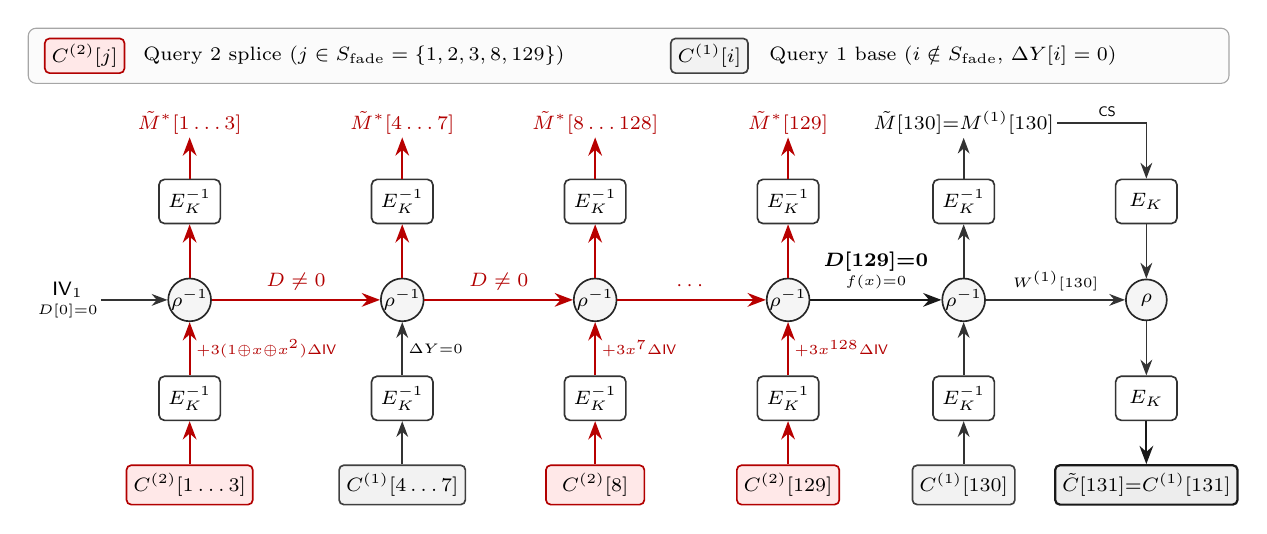
\begin{tikzpicture}[
    >=Stealth,
    bcinv/.style={rectangle, draw=black!80, semithick, rounded corners=0.7mm, fill=white, minimum width=7.8mm, minimum height=5.6mm, inner sep=1pt, font=\scriptsize\bfseries},
    bcfwd/.style={rectangle, draw=black!80, semithick, rounded corners=0.7mm, fill=white, minimum width=7.8mm, minimum height=5.6mm, inner sep=1pt, font=\scriptsize\bfseries},
    c1box/.style={rectangle, draw=black!75, semithick, rounded corners=0.6mm, fill=gray!10, minimum width=12.5mm, minimum height=5.0mm, inner ysep=1pt, inner xsep=2.5pt, font=\scriptsize},
    c2box/.style={rectangle, draw=red!70!black, semithick, rounded corners=0.6mm, fill=red!9, minimum width=12.5mm, minimum height=5.0mm, inner ysep=1pt, inner xsep=2.5pt, font=\scriptsize\bfseries},
    rhoinv/.style={circle, draw=black!85, semithick, fill=gray!8, minimum size=5.2mm, inner sep=0pt, font=\scriptsize},
    lbl/.style={font=\scriptsize, inner sep=1pt},
    wire/.style={->, semithick, draw=black!80},
    diffwire/.style={->, thick, draw=red!72!black},
    zerowire/.style={->, thick, draw=black!90}
]

% Legend at top
\draw[rounded corners=1mm, draw=black!35, fill=gray!3] (0.0, 2.75) rectangle (15.25, 3.45);
\node[c2box, minimum width=9.5mm, minimum height=4.4mm, anchor=west] at (0.20, 3.10) {$C^{(2)}[j]$};
\node[lbl, anchor=west] at (1.42, 3.10) {Query~2 splice ($j \in S_{\mathrm{fade}} = \{1, 2, 3, 8, 129\}$)};
\node[c1box, minimum width=9.5mm, minimum height=4.4mm, anchor=west] at (8.15, 3.10) {$C^{(1)}[i]$};
\node[lbl, anchor=west] at (9.37, 3.10) {Query~1 base ($i \notin S_{\mathrm{fade}}$, $\Delta Y[i] = 0$)};

% Entry IV_1
\node[lbl, align=center] (iv1) at (0.50, 0.0) {$\IV_1$\\[-1pt]{\tiny $D[0]{=}0$}};

% Column 1: j in {1,2,3} (x = 2.05)
\node[c2box] (in1) at (2.05, -2.35) {$C^{(2)}[1 \dots 3]$};
\node[bcinv] (le1) at (2.05, -1.25) {$E_K^{-1}$};
\node[rhoinv](r1)  at (2.05,  0.00) {$\rho^{-1}$};
\node[bcinv] (ue1) at (2.05,  1.25) {$E_K^{-1}$};
\node[lbl, text=red!70!black] (m1) at (2.05, 2.25) {$\tilde{M}^*[1 \dots 3]$};

\draw[wire]     (iv1) -- (r1);
\draw[diffwire] (in1) -- (le1);
\draw[diffwire] (le1) -- node[lbl, right=1pt, text=red!70!black] {\tiny $+3(1{\oplus}x{\oplus}x^2)\Delta\IV$} (r1);
\draw[diffwire] (r1) -- (ue1);
\draw[diffwire] (ue1) -- (m1);

% Column 2: i in {4..7} (x = 4.75)
\node[c1box] (in2) at (4.75, -2.35) {$C^{(1)}[4 \dots 7]$};
\node[bcinv] (le2) at (4.75, -1.25) {$E_K^{-1}$};
\node[rhoinv](r2)  at (4.75,  0.00) {$\rho^{-1}$};
\node[bcinv] (ue2) at (4.75,  1.25) {$E_K^{-1}$};
\node[lbl, text=red!70!black] (m2) at (4.75, 2.25) {$\tilde{M}^*[4 \dots 7]$};

\draw[diffwire] (r1) -- node[lbl, above=2pt, text=red!70!black] {$D \neq 0$} (r2);
\draw[wire] (in2) -- (le2);
\draw[wire] (le2) -- node[lbl, right=1pt] {\tiny $\Delta Y{=}0$} (r2);
\draw[diffwire] (r2) -- (ue2);
\draw[diffwire] (ue2) -- (m2);

% Column 3: j = 8 & 9..128 (x = 7.20)
\node[c2box] (in3) at (7.20, -2.35) {$C^{(2)}[8]$};
\node[bcinv] (le3) at (7.20, -1.25) {$E_K^{-1}$};
\node[rhoinv](r3)  at (7.20,  0.00) {$\rho^{-1}$};
\node[bcinv] (ue3) at (7.20,  1.25) {$E_K^{-1}$};
\node[lbl, text=red!70!black] (m3) at (7.20, 2.25) {$\tilde{M}^*[8 \dots 128]$};

\draw[diffwire] (r2) -- node[lbl, above=2pt, text=red!70!black] {$D \neq 0$} (r3);
\draw[diffwire] (in3) -- (le3);
\draw[diffwire] (le3) -- node[lbl, right=1pt, text=red!70!black] {\tiny $+3x^7\Delta\IV$} (r3);
\draw[diffwire] (r3) -- (ue3);
\draw[diffwire] (ue3) -- (m3);

% Column 4: j = 129 FADE POINT (x = 9.65)
\node[c2box] (in4) at (9.65, -2.35) {$C^{(2)}[129]$};
\node[bcinv] (le4) at (9.65, -1.25) {$E_K^{-1}$};
\node[rhoinv](r4)  at (9.65,  0.00) {$\rho^{-1}$};
\node[bcinv] (ue4) at (9.65,  1.25) {$E_K^{-1}$};
\node[lbl, text=red!70!black] (m4) at (9.65, 2.25) {$\tilde{M}^*[129]$};

\draw[diffwire] (r3) -- node[lbl, above=2pt, text=red!70!black] {$\cdots$} (r4);
\draw[diffwire] (in4) -- (le4);
\draw[diffwire] (le4) -- node[lbl, right=1pt, text=red!70!black] {\tiny $+3x^{128}\Delta\IV$} (r4);
\draw[diffwire] (r4) -- (ue4);
\draw[diffwire] (ue4) -- (m4);

% Column 5: i = 130 Checksum Block (x = 11.88)
\node[c1box] (in5) at (11.88, -2.35) {$C^{(1)}[130]$};
\node[bcinv] (le5) at (11.88, -1.25) {$E_K^{-1}$};
\node[rhoinv](r5)  at (11.88,  0.00) {$\rho^{-1}$};
\node[bcinv] (ue5) at (11.88,  1.25) {$E_K^{-1}$};
\node[lbl, align=center] (m5) at (11.88, 2.25) {$\tilde{M}[130]{=}M^{(1)}[130]$};

\draw[zerowire] (r4) -- node[lbl, above=2.5pt, align=center] {{\boldmath $D[129]{=}0$}\\[-1pt]{\tiny $f(x){=}0$}} (r5);
\draw[wire] (in5) -- (le5);
\draw[wire] (le5) -- (r5);
\draw[wire] (r5) -- (ue5);
\draw[wire] (ue5) -- (m5);

% Column 6: i = 131 Tag Verification (x = 14.20)
\node[bcfwd] (ue6) at (14.20,  1.25) {$E_K$};
\node[rhoinv](r6)  at (14.20,  0.00) {$\rho$};
\node[bcfwd] (le6) at (14.20, -1.25) {$E_K$};
\node[c1box, draw=black!90, thick, fill=gray!14, font=\scriptsize\bfseries] (in6) at (14.20, -2.35) {$\tilde{C}[131]{=}C^{(1)}[131]$};

\draw[wire] (r5) -- node[lbl, above=2pt] {\tiny $W^{(1)}[130]$} (r6);
\draw[wire] (m5.east) -| node[lbl, above=1pt, pos=0.28] {\tiny $\CS$} (ue6.north);
\draw[wire] (ue6) -- (r6);
\draw[wire] (r6) -- (le6);
\draw[zerowire] (le6) -- (in6);

\end{tikzpicture}
\caption{Decryption dataflow of the two-query nonce-respecting Difference-Fade forgery $\mathsf{COLM}_0\text{-}\mathsf{Dec}_K(N_1, A_1, C^{\mathrm{mix}})$ at $\ell = 130$ (Theorem~\ref{thm:fade}; masking XORs omitted for clarity). Splicing $C^{(2)}[j]$ at $S_{\mathrm{fade}} = \{1, 2, 3, 8, 129\}$ injects $3\,\Delta\IV\,(1 \oplus x \oplus x^2 \oplus x^7 \oplus x^{128}) = 3\,\Delta\IV \cdot f(x) = 0$ into the chaining difference $D[129]$, restoring $W_{\mathrm{mix}}[129] = W^{(1)}[129]$ while checksum telescoping (Lemma~\ref{lem:telescoping}) shields tag verification from all modified plaintext blocks $\tilde{M}^*[1 \dots 129]$.}
\label{fig:fade-attack}
\end{figure}

\begin{theorem}[Two-Query Nonce-Respecting Difference-Fade Forgery on $\COLMzero$]
\label{thm:fade}
Let $\ell \ge 130$ be any integer, let $M$ be any block-aligned plaintext of $\ell$ blocks ($16\ell$ bytes), and let $(N_1, A_1), (N_2, A_2)$ be any two pairs with $N_1 \neq N_2$ (nonce-respecting). Given the two ciphertexts $C^{(1)} \leftarrow \mathsf{COLM}_0\text{-}\mathsf{Enc}_K(N_1, A_1, M)$ and $C^{(2)} \leftarrow \mathsf{COLM}_0\text{-}\mathsf{Enc}_K(N_2, A_2, M)$, define the $5$-element splice index set
\begin{equation}
\label{eq:S-fade}
S_{\mathrm{fade}} := \supp\big(f(x)\big) + 1 = \{1, 2, 3, 8, 129\}.
\end{equation}
Then the spliced ciphertext $C^{\mathrm{mix}}$ defined by~\eqref{eq:c-mix} with $S = S_{\mathrm{fade}}$ is accepted by the verification routine $\mathsf{COLM}_0\text{-}\mathsf{Dec}_K(N_1, A_1, C^{\mathrm{mix}})$ with probability~$1$ (provided $\IV_1 \neq \IV_2$, which holds deterministically for every key $K$ whenever $A_1 = A_2$ by the bijectivity of $E_K$). Moreover, $\ell_{\min} = 130$ is the strict minimum block length for which any non-empty fade splice exists.
\end{theorem}

\begin{proof}
Since $M^{(1)} = M^{(2)} = M$ and $\max(S_{\mathrm{fade}}) = 129 \le \ell - 1$, the internal message blocks $M^{(1)}[i]$ and $M^{(2)}[i]$ coincide for all $1 \le i \le \ell$. By~\eqref{eq:D-poly}, at every block $i \in \{129, \dots, \ell - 1\}$, the chaining-state difference is
\begin{equation}
D[i] = 3 \, \Delta\IV \cdot \sum_{j \in \{1, 2, 3, 8, 129\}} x^{j-1} = 3 \, \Delta\IV \cdot \big(1 \oplus x \oplus x^2 \oplus x^7 \oplus x^{128}\big) = 3 \, \Delta\IV \cdot f(x) = 0 \quad \text{in } \FtwoN.
\end{equation}
In particular, $D[\ell - 1] = 0$, so $W_{\mathrm{mix}}[\ell - 1] = W^{(1)}[\ell - 1]$. Because $C^{\mathrm{mix}}[\ell] = C^{(1)}[\ell]$ and $C^{\mathrm{mix}}[\ell + 1] = C^{(1)}[\ell + 1]$ ($129 < \ell < \ell + 1$), Lemma~\ref{lem:telescoping} implies that $\tilde{M}_{\mathrm{mix}}[\ell] = M^{(1)}[\ell]$ and $W_{\mathrm{mix}}[\ell] = W^{(1)}[\ell]$. The recomputed tag block $\tilde{C}^{\mathrm{mix}}[\ell + 1]$ therefore equals $C^{(1)}[\ell + 1] = C^{\mathrm{mix}}[\ell + 1]$ identically. Whenever $\Delta\IV \neq 0$, $Y^{(1)}[j] \neq Y^{(2)}[j]$ for all $j \in S_{\mathrm{fade}}$, so $C^{\mathrm{mix}} \neq C^{(1)}$ and $C^{\mathrm{mix}} \neq C^{(2)}$ is a valid, non-trivial $\mathsf{INT\text{-}CTXT}$ forgery.

To see that $\ell_{\min} = 130$ is tight, note that retaining the tag block $C^{\mathrm{mix}}[\ell+1] = C^{(1)}[\ell+1]$ requires both $\tilde{M}_{\mathrm{mix}}[\ell] = M^{(1)}[\ell]$ (hence $X_{\mathrm{mix}}[\ell] = X^{(1)}[\ell]$) and $W_{\mathrm{mix}}[\ell] = W^{(1)}[\ell]$. Since $\rho^{-1}$ is a bijection, this forces $Y_{\mathrm{mix}}[\ell] = Y^{(1)}[\ell]$ and $W_{\mathrm{mix}}[\ell-1] = W^{(1)}[\ell-1]$ ($D[\ell-1] = 0$), so index $\ell$ cannot belong to $S$. Thus $S \subseteq \{1, \dots, \ell - 1\}$, and $\sum_{j \in S} x^{j-1} = 0$ requires a non-trivial $\Ftwo$-linear dependency among $\{x^0, x^1, \dots, x^{\ell-2}\}$. Because $\deg(f) = 128$, the powers $\{1, x, \dots, x^{127}\}$ form a basis of $\FtwoN$ over $\Ftwo$, so $\rank_{\Ftwo}\{x^0, \dots, x^{\ell-2}\} = \ell - 1$ for all $\ell \le 129$. The first dependency therefore occurs at $\ell - 2 = 128$, i.e., $\ell_{\min} = 130$.
\end{proof}

\subsection{Mechanism 2: State-Transfer Forgery (\texorpdfstring{$\ell \ge 129$}{l >= 129})}
Instead of fading $D[\ell-1]$ back to zero and reusing Query~1's tag block, our second forgery family drives the spliced chaining state $W_{\mathrm{mix}}$ onto \emph{Query~2's chaining state $W^{(2)}$} and transplants Query~2's final block and tag block (generalizing the fixed-$\IV$ intermediate-tag splice of Datta and Nandi~\cite[Section~5.2]{DN14} to distinct nonces and full-message checksum tags on $\COLMzero$).

\begin{theorem}[Two-Query Nonce-Respecting State-Transfer and Tag-Transplant Forgery on $\COLMzero$]
\label{thm:transplant}
Let $\ell \ge 129$ be any integer, let $m \in \{129, \dots, \ell\}$ be any run-start index, and let $C^{(1)}, C^{(2)}$ be the ciphertexts of the same $\ell$-block message $M$ under distinct nonces $N_1 \neq N_2$. Define the splice index set
\begin{equation}
\label{eq:S-transplant}
S_{\mathrm{trans}}(\ell, m) := \Big(\supp\big(3^{-1} x^{m-1}\big) + 1\Big) \;\cup\; \{m, m + 1, \dots, \ell + 1\}.
\end{equation}
At the minimal length $\ell = m = 129$ blocks ($2{,}064$~bytes), $S_{\mathrm{trans}}(129, 129)$ is the $8$-element set
\begin{equation}
\label{eq:S-trans-129}
S_{\mathrm{trans}}(129, 129) = \{1, 3, 4, 5, 6, 7, 129, 130\}.
\end{equation}
Then $C^{\mathrm{mix}}$ spliced on $S = S_{\mathrm{trans}}(\ell, m)$ is accepted by $\mathsf{COLM}_0\text{-}\mathsf{Dec}_K(N_1, A_1, C^{\mathrm{mix}})$ with probability~$1$ (provided $\IV_1 \neq \IV_2$, which holds deterministically whenever $A_1 = A_2$), and $\ell_{\min} = 129$ is the strict minimum block length of this family.
\end{theorem}

\begin{proof}
Observe first that splicing block $i$ ($i \in S$, so $Y_{\mathrm{mix}}[i] = Y^{(2)}[i]$) makes the decrypted upper-layer state $X_{\mathrm{mix}}[i] = Y^{(2)}[i] \oplus 3W_{\mathrm{mix}}[i-1]$ and updated chaining state $W_{\mathrm{mix}}[i] = Y^{(2)}[i] \oplus W_{\mathrm{mix}}[i-1]$ equal to Query~2's states $(X^{(2)}[i], W^{(2)}[i])$. This holds if and only if $W_{\mathrm{mix}}[i-1] = W^{(2)}[i-1]$. Once $W_{\mathrm{mix}}[m-1] = W^{(2)}[m-1]$ holds at index $m - 1$, splicing every subsequent block $i \in \{m, m + 1, \dots, \ell + 1\}$ inductively maintains $W_{\mathrm{mix}}[i] = W^{(2)}[i]$ and $\tilde{M}_{\mathrm{mix}}[\ell] = M^{(2)}[\ell]$. The transplanted tag block $C^{\mathrm{mix}}[\ell + 1] = C^{(2)}[\ell + 1]$ therefore verifies under $(N_1, A_1)$ with probability~$1$.

By~\eqref{eq:W12-diff} and~\eqref{eq:D-poly}, the state-transfer condition $W_{\mathrm{mix}}[m-1] = W^{(2)}[m-1]$ is equivalent to $D[m-1] = W^{(1)}[m-1] \oplus W^{(2)}[m-1] = x^{m-1} \Delta\IV$, which holds for all $\Delta\IV$ if and only if
\begin{equation}
\label{eq:transplant-cond}
3 \sum_{\substack{j \in S \\ j \le m - 1}} x^{j-1} = x^{m-1} \quad \Longleftrightarrow \quad \sum_{\substack{j \in S \\ j \le m - 1}} x^{j-1} = 3^{-1} x^{m-1} \quad \text{in } \FtwoN.
\end{equation}
Since $S \cap \{1, \dots, m - 1\}$ can only use exponents $\{0, 1, \dots, m - 2\}$, equation~\eqref{eq:transplant-cond} admits a solution if and only if
\begin{equation}
\label{eq:cond-C}
\deg\big(3^{-1} x^{m-1} \bmod f(x)\big) \le m - 2 \qquad \text{(Condition~C)}.
\end{equation}
In $\FtwoN = \Ftwo[x]/(x^{128} + x^7 + x^2 + x + 1)$, the element $(x + 1)^{-1} = x \oplus \sum_{k=7}^{127} x^k$ has degree $127$. Direct computation shows that $\deg(3^{-1} x^{m-1} \bmod f) = 127 > m - 2$ for every $1 \le m \le 128$. At $m = 129$, $3^{-1} x^{128} = 3^{-1}(x^7 \oplus x^2 \oplus x \oplus 1) = x^6 \oplus x^5 \oplus x^4 \oplus x^3 \oplus x^2 \oplus 1$, which has degree $6 \le 127$ and support $\{0, 2, 3, 4, 5, 6\}$. Shifting indices by $+1$ gives the prefix $\{1, 3, 4, 5, 6, 7\}$, and adjoining the contiguous suffix $\{129, \dots, \ell+1\}$ yields~\eqref{eq:S-transplant}--\eqref{eq:S-trans-129}.
\end{proof}

\subsection{Extensions and Comparison with Nonce-Misuse Splicing}
\label{subsec:generalisations}
The algebraic framework of~\eqref{eq:D-general}--\eqref{eq:D-poly} yields three additional observations:
\begin{enumerate}[leftmargin=2em]
    \item \textbf{Common-Prefix Relaxation:} In Theorem~\ref{thm:fade}, the two queried messages $M^{(1)}$ (of length $\ell_1 \ge 130$ blocks) and $M^{(2)}$ (of any length $\ell_2 \ge 130$ blocks, including messages with an incomplete final block) need \emph{not} be identical. They only need to agree on their first $129$ blocks ($M^{(1)}[1 \dots 129] = M^{(2)}[1 \dots 129]$, a $2{,}064$-byte common prefix). Because $\max(S_{\mathrm{fade}}) = 129$, decryption of $C^{\mathrm{mix}}$ never accesses $C^{(2)}[i]$ for $i \ge 130$.
    \item \textbf{Same-Nonce / Distinct-AD Relaxation:} Because $W[0] = \IV$ is a function of $(N, A)$, the condition $\Delta\IV \neq 0$ in Theorems~\ref{thm:fade} and~\ref{thm:transplant} is satisfied whenever the two queries use distinct nonces under arbitrary associated data (including empty or non-block-aligned $\AD$). It is equally satisfied when they repeat a nonce under distinct associated data $A_1 \neq A_2$.
    \item \textbf{Incompatibility with First-Block Message Differences:} If two queries also differ in the first plaintext block ($M^{(1)}[1] \neq M^{(2)}[1]$, inducing an upper-layer difference $\delta = X^{(1)}[1] \oplus X^{(2)}[1] \neq 0$) while agreeing on blocks $2, \dots, \ell$, then splicing requires $\Delta\IV = 0$ (the nonce-reuse setting of~\cite{DN14,DLMN17}):
\end{enumerate}

\begin{proposition}[Two-Query Splicing with a First-Block Message Difference]
\label{prop:case-c}
Let Query~1 and Query~2 agree on plaintext blocks $2, \dots, \ell$ ($\ell \ge 130$), with initial chaining difference $\Delta\IV = \IV_1 \oplus \IV_2$ and block-$1$ upper-layer difference $\delta = X^{(1)}[1] \oplus X^{(2)}[1]$. Then for any splice set $S \subseteq \{1, \dots, 129\}$, the chaining difference at block $129$ is
\begin{equation}
\label{eq:D-two-unknowns}
D[129] = \Big(\mathbf{1}_{[1 \in S]} \oplus 3u\Big) \delta \;\oplus\; 3\Big(\mathbf{1}_{[1 \in S]} \oplus 2u\Big) \Delta\IV, \qquad \text{where } u = \sum_{\substack{j \in S \\ j \ge 2}} x^{j-2} \in \FtwoN.
\end{equation}
In particular, when $\Delta\IV = 0$ and $\delta \neq 0$ (nonce reuse), $D[129] = 0$ holds if and only if $1 \in S$ and $u = 3^{-1}$, recovering the $123$-element $3^{-1}$-expansion splice set $S_B = \{1\} \cup \{i + 2 : \mathsf{bit}_i(3^{-1}) = 1\}$ of Datta et al.~\cite[Lemma~2]{DLMN17} (or the $5$-element shifted set $S_{\mathrm{fade}} + 1 = \{2, 3, 4, 9, 130\}$ at $\ell \ge 131$). Conversely, when both $\Delta\IV \neq 0$ and $\delta \neq 0$, canceling the two independent pseudorandom values $\delta$ and $\Delta\IV$ requires $\mathbf{1}_{[1 \in S]} \oplus 3u = 0$ and $\mathbf{1}_{[1 \in S]} \oplus 2u = 0$, which forces $u = 0$, $\mathbf{1}_{[1 \in S]} = 0$, and hence $S = \emptyset$.
\end{proposition}

\section{Analysis of the Official Security Proofs}
\label{sec:proof-flaw}

Two security proofs have been published by the $\COLM$ designers for $\COLMzero$ ($\tau = 0$):
\begin{enumerate}[leftmargin=2em]
    \item \textbf{The 2024 \emph{Journal of Cryptology} Proof~\cite[Section~4, pp.~15--25]{COLM24}:} A full Patarin H-coefficient proof for unified online authenticated encryption ($\mathsf{oAE}$) security (Theorem~2, Lemma~1, Lemma~2, and Section~4.4).
    \item \textbf{The 2016 CAESAR Round-3 Addendum~\cite[Section~2, pp.~2--4]{COLMadd}:} An H-coefficient proof bounding the forgery advantage $\Adv^{\mathrm{auth}}_{\COLM_\Pi}$ (Theorem~2, Lemma~3, and Lemma~4).
\end{enumerate}
We evaluate both theorems at the parameters of our two-query adversary ($q = 2$ forward encryption queries, $s = 1$ forgery attempt, and zero prior decryption/RUP queries). We then identify the exact mathematical steps at which each proof breaks down against this two-query adversary.

\subsection{The 2024 \emph{Journal of Cryptology} Security Proof}
Theorem~2 of~\cite[Section~4, p.~15]{COLM24} states verbatim:
\begin{quote}
\itshape
``\textbf{Theorem 2.} Let us consider an adversary $\mathcal{A}$ that makes $q$ encryption queries and $s$ forging attempts at an overall aggregate of total $a$ associated data and $m$ message blocks and tries to distinguish $\COLMzero$ from a random online function. Let $\sigma = a + 2m + 3(q + s)$. The $\mathsf{oAE}$ advantage of $\COLMzero$ is given by
\begin{equation}
\label{eq:joc2024-thm2}
\Adv^{\mathsf{oAE}}_{\COLMzero}(\mathcal{A}) \le \Adv^{\mathsf{SPRP}}_E(\mathcal{A}') + \frac{7\sigma^2 + 3\sigma + qs + 3s + 2s\sigma}{2^n}\text{,''}
\end{equation}
\end{quote}
where Lemma~2~\cite[p.~23]{COLM24} bounds the probability of bad transcripts by $\epsilon_{\mathrm{bad}} \le (7\sigma^2 + 3\sigma + qs)/2^n$, and Section~4.4~\cite[pp.~24--25]{COLM24} bounds the good-transcript forgery ratio by $\epsilon_{\mathrm{ratio}} \le (3s + 2s\sigma)/2^n$.

At our adversary's parameters ($n = 128$, $q = 2$, $s = 1$, $a_i \le 2$ giving $a \le 6$, and $\ell_i \in \{129, 130\}$ giving $m \le 390$), we have $\sigma = a + 2m + 3(q + s) \le 6 + 780 + 9 = 795$. Substituting $\sigma = 795$ into~\eqref{eq:joc2024-thm2} gives the claimed information-theoretic bound
\begin{equation}
\label{eq:joc2024-eval}
\epsilon_{\mathrm{bad}} + \epsilon_{\mathrm{ratio}} = \frac{7(795)^2 + 3(795) + 2 + 3 + 2(795)}{2^{128}} = \frac{4{,}428{,}155}{2^{128}} \approx 2^{-105.92},
\end{equation}
whereas our adversary achieves $\Adv^{\mathsf{oAE}}_{\COLMzero}(\mathcal{A}) = 1$, exceeding the claimed bound by a factor of $2^{105.92}$.

\paragraph{Flaw 1: Checksum Direction Inversion in Event $\mathsf{BadSamp}$.}
In the 2024 proof, Bad Event~$\mathsf{B6}$~\cite[p.~22]{COLM24} is defined as the event that a non-trivial decryption query $i \in \mathcal{D}$ has \emph{no} fresh upper-layer output block $X_i^-[j]$ across all $1 \le j \le \ell_i$:
\begin{equation}
\mathsf{B6} \;:\; \exists i \in \mathcal{D} \;\text{ s.t. }\; X_i^-[j] = X_{i_j}^+[j] \quad \forall j \le \ell_i.
\end{equation}
In our Difference-Fade forgery (Theorem~\ref{thm:fade}, $\ell = 130$), the spliced blocks $S_{\mathrm{fade}} = \{1, 2, 3, 8, 129\}$ alter the intermediate chaining states $W_{\mathrm{mix}}[j]$ for $1 \le j \le 128$. Hence, $X_i^-[j] = Y^{(2)}[j] \oplus 3W_{\mathrm{mix}}[j-1]$ is genuinely \emph{fresh} for $j \in \{1, \dots, 128\}$. Bad Event~$\mathsf{B6}$ therefore does not occur, and the transcript satisfies the good-transcript definition of Section~4.3.

Next, in Section~4.4 (\emph{Calculation of $\epsilon_{\mathrm{ratio}}$}~\cite[p.~24]{COLM24}), the authors bound the conditional forgery probability $\epsilon_i = \Pr[\mathsf{Forge}_i \mid \tau_e, \tau_d]$ on a good transcript. They argue verbatim:
\begin{quote}
\itshape
``By the properties of a good transcript, the set $\{j : X_i^-[j] \text{ is fresh}\}$ is nonempty. Let $j_i$ denote the smallest such index. Now we sample all $MM_i^-[k]$ values randomly in without replacement manner from $\{0,1\}^n \setminus \mathcal{O}$, where $k \in \{j : X_i^-[j] \text{ is fresh}\}$. All other $MM_i^-[j]$ values are set\dots\ Now we say that the sampling of $MM_i^-$ values is bad, denoted by the event $\mathsf{BadSamp}$, if $MM_i^-[\ell_i]$ is not fresh, i.e., $MM_i^-[\ell_i] \in \mathcal{I} \cup \{MM_i^-[j] : j < \ell_i\}$. It is easy to see that the probability of the event $\mathsf{BadSamp}$ is bounded by $1/(2^n - 2\sigma)$ \emph{due to the randomness of $MM_i^-[j_i]$} \textup{[emphasis added]}. Now conditioned on the event that $\mathsf{BadSamp}$ does not occur, we can sample distinct values of $CC_i^-[\ell_i + 1]$ uniformly at random\dots''
\end{quote}
This step contains a direction-inversion error between encryption and decryption:
\begin{itemize}[leftmargin=2em]
    \item The proof implicitly assumes that in a decryption query $i \in \mathcal{D}$, the $\ell_i$-th internal block $MM_i^-[\ell_i]$ (and thus the $(\ell_i+1)$-th input $M_i^-[\ell_i+1] = M_i^-[\ell_i]$ governing the tag $CC_i^-[\ell_i+1]$) incorporates the XOR sum of the preceding decrypted blocks $M_i^-[1] \oplus \dots \oplus M_i^-[\ell_i-1]$. That sum would inherit the randomness of $MM_i^-[j_i]$ ($j_i = 1 < \ell_i$).
    \item In fact, according to the decryption specification $\COLMzero.\mathsf{dec}$~\cite[Figure~3, p.~12]{COLM24}, $MM_i^-[\ell_i] = E_K^{-1}(X_i^-[\ell_i])$ and $M_i^-[\ell_i] = MM_i^-[\ell_i] \oplus \Delta_2[\ell_i]$ (denoted $\Delta_M[\ell_i]$ in Section~\ref{sec:spec}) are determined \emph{solely} by the $\ell_i$-th ciphertext block $C_i^-[\ell_i]$ and the incoming chaining state $W_i^-[\ell_i-1]$ via $X_i^-[\ell_i] = Y_i^-[\ell_i] \oplus 3W_i^-[\ell_i-1]$. The preceding blocks $M_i^-[1 \dots \ell_i-1]$ are XORed only into the external output plaintext block $M_i^\star[\ell_i] \leftarrow M_i^-[1] \oplus \dots \oplus M_i^-[\ell_i]$. The tag-generation input, by contrast, is set to $M_i^-[\ell_i+1] \leftarrow M_i^-[\ell_i]$ rather than $M_i^\star[\ell_i]$.
    \item In our Difference-Fade forgery ($\ell_i = 130$), $D[129] = 0$ ensures $W_i^-[129] = W_1^+[129]$, while $C_i^-[130] = C_1^+[130]$ ensures $Y_i^-[130] = Y_1^+[130]$. As a result, $X_i^-[130] = X_1^+[130]$ is \emph{not fresh}, forcing $MM_i^-[130] = MM_1^+[130]$ and $CC_i^-[131] = CC_1^+[131]$ with probability~$1$, independently of $MM_i^-[j_i]$.
\end{itemize}

\paragraph{Flaw 2: Overlooking $\FtwoN$ Polynomial Dependencies in Lemma~1.}
In our State-Transfer forgery (Theorem~\ref{thm:transplant}, $\ell_i = 129$) and in the second subcase of Bad Event~$\mathsf{B6}$ (``$\forall j, CC_i^-[j]$ is not fresh''~\cite[p.~23]{COLM24}), every ciphertext block of $C_i^-$ is copied from either Query~1 or Query~2 at the corresponding block index $j$. To argue that $L_X(W[0], Y[1 \mathinner{..} j+1])$ cannot coincide with $X'[j+1]$, the authors invoke Lemma~1~\cite[p.~20]{COLM24}, expanding $L_X(W[0], Y[1 \mathinner{..} j+1])$ as
\begin{equation}
L_X(W[0], Y[1 \mathinner{..} j{+}1]) = X'[j{+}1] \oplus 3(X[j] \oplus X'[j]) \oplus \dots \oplus 3 \cdot 2^{j-1}(X'[1] \oplus X[1]) \oplus 3 \cdot 2^j(W'[0] \oplus W[0]),
\end{equation}
and concluding that equality with $X'[j+1]$ forces $W'[0] \equiv W[0]$ and $X'[r] \equiv X[r]$ for all $r$. This implication fails for $\ell_i \ge 129$. When two queries share a $129$-block plaintext prefix, $X_1^+[r] \equiv X_2^+[r]$ already holds for $1 \le r \le 128$. The accumulated initial-value terms $\Delta W[0] = W_1^+[0] \oplus W_2^+[0]$ across $S$ then sum to $\big(3 \sum_{r \in S, r \le 128} 2^{r-1} \oplus 2^{128}\big) \Delta W[0]$. That sum vanishes identically in $\FtwoN$ whenever $S \cap \{1, \dots, 128\} = \supp(3^{-1} 2^{128}) + 1 = \{1, 3, 4, 5, 6, 7\}$, despite $W_1^+[0] \neq W_2^+[0]$.

\subsection{The 2016 CAESAR Round-3 Addendum Proof}
In the earlier 2016 CAESAR Round-3 addendum~\cite[Section~2, p.~3]{COLMadd}, Theorem~2 claims that for $\sigma = \sum_{i=1}^{q+s} (a_i + \ell_i)$ and $\sigma_{\mathrm{auth}} = \sigma + q$,
\begin{equation}
\label{eq:thm2-bound}
\Adv^{\mathrm{auth}}_{\COLM_\Pi}(\mathcal{A}) \le \frac{9\sigma_{\mathrm{auth}}^2}{2^n} + \frac{s}{2^n}.
\end{equation}
At $q = 2, s = 1, a_i = 2, \ell_i = 130$ ($\sigma = 396, \sigma_{\mathrm{auth}} = 398$),~\eqref{eq:thm2-bound} evaluates to $2^{-107.56}$. In that proof, Step~I (Condition~2~\cite[p.~3]{COLMadd}) defines a ``good online forge view'' ($\tau_{\mathrm{good}}$) by requiring that for every forgery attempt $j > q$, the submitted tag block $C_j[\ell_j + 1]$ be \emph{fresh} (``distinct and different from all other $C_i[j']$'s''). Lemma~3 then bounds $\Pr[\tau \notin \tau_{\mathrm{good}}] \le \frac{(q + \sum_{i=1}^q \ell_i)^2}{2^{n+1}} + \frac{s(q + s + \sigma)}{2^n} = \frac{34{,}721}{2^{128}} \approx 2^{-112.92}$ (further upper-bounded by $2\sigma_{\mathrm{auth}}^2 / 2^n \approx 2^{-109.73}$) in the ideal world, while Lemma~4~\cite[pp.~3--4]{COLMadd} lower-bounds the real-world interpolation ratio by claiming that choosing fresh intermediate blocks $MM$ yields fresh checksums and fresh final $Y$ blocks. This argument fails for the same two reasons identified above: in $\COLMzero$, checksum telescoping decouples the tag input $M_3[\ell+1] = M_3[\ell]$ from intermediate blocks $MM_3[1 \dots \ell-1]$, and aligning $W_{\mathrm{mix}}[\ell-1]$ with $W^{(1)}[\ell-1]$ (Theorem~\ref{thm:fade}) or $W^{(2)}[\ell-1]$ (Theorem~\ref{thm:transplant}) allows the adversary to reuse $C_3[\ell+1] := C_1[\ell+1]$ or $C_2[\ell+1]$ deterministically.

\section{Resistance of \texorpdfstring{$\COLMott$}{COLM\_127} and Mode-Level Mitigations}
\label{sec:repair}

Recall from Section~\ref{sec:attack} that our two-query nonce-respecting forgeries on $\COLMzero$ rely on the simultaneous presence of three structural properties:
(i)~an uninterrupted chaining horizon of at least $129$ message blocks, allowing the degree-$128$ field polynomial $f(x)$ to cancel $\Delta\IV$;
(ii)~a nonce-independent upper-layer mask base $\Delta_1 = L$, allowing $X^{(1)}[i] = X^{(2)}[i]$ to cancel across distinct nonces; and
(iii)~an unweighted duplicate checksum $M[\ell+1] = M[\ell] = \bigoplus_{i=1}^\ell M^*[i]$, allowing intermediate plaintext corruptions to telescope out during decryption (Lemma~\ref{lem:telescoping}).
As illustrated in Figure~\ref{fig:colm-mitigations}, breaking any one of these three links prevents two-query splicing. We first analyze how $\COLMott$ ($\tau = 127$, \textbf{Modification~1}) truncates the chaining horizon one block before the degree-$128$ threshold, and then evaluate two zero-expansion mode-level modifications (\textbf{Modifications~2 and~3}).

\begin{figure}[t!]
\centering
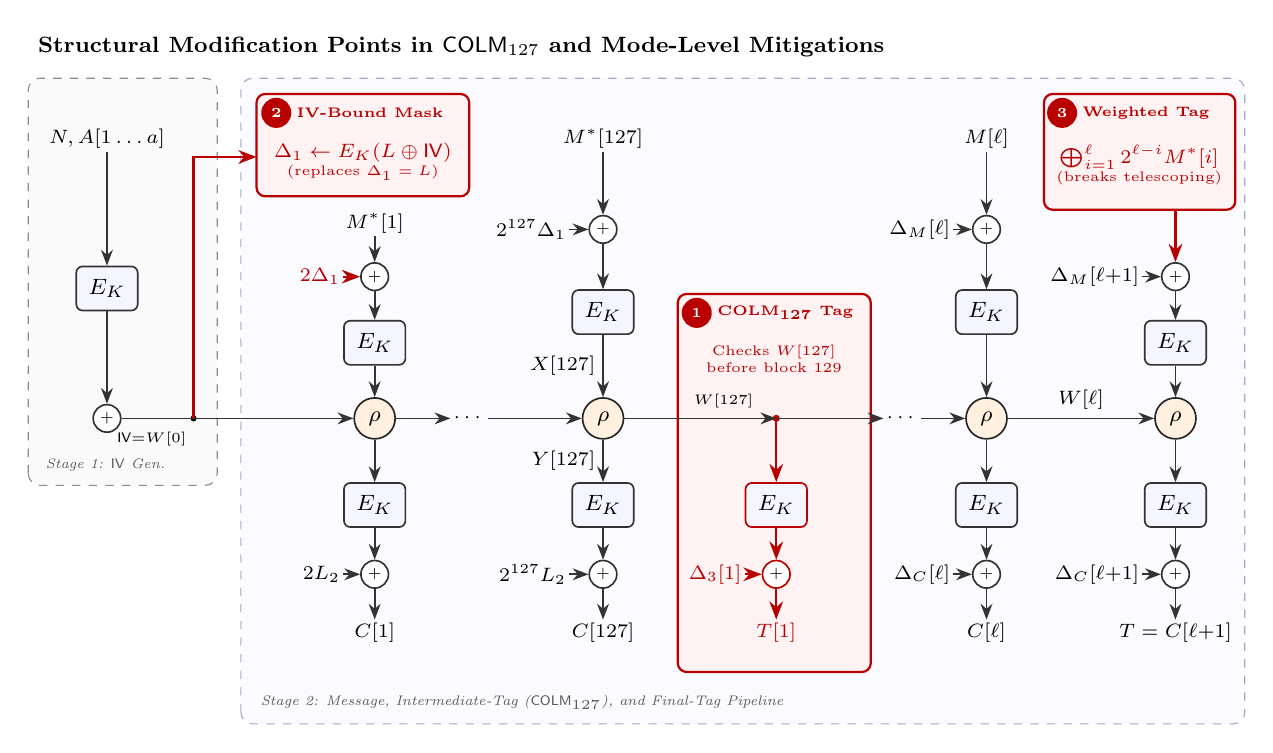
\begin{tikzpicture}[
    >=Stealth,
    bc/.style={rectangle, draw=black!80, semithick, rounded corners=0.8mm, fill=blue!4, minimum width=7.8mm, minimum height=5.6mm, inner sep=1pt, font=\footnotesize\bfseries},
    xor/.style={circle, draw=black!80, semithick, fill=white, minimum size=3.5mm, inner sep=0pt, font=\tiny},
    rhonode/.style={circle, draw=black!85, semithick, fill=orange!12, minimum size=5.2mm, inner sep=0pt, font=\footnotesize},
    modbox/.style={rounded corners=1.1mm, draw=red!72!black, thick, fill=red!5},
    modbadge/.style={circle, draw=red!72!black, semithick, fill=red!72!black, text=white, minimum size=3.6mm, inner sep=0pt, font=\tiny\bfseries},
    lbl/.style={font=\scriptsize, inner sep=1pt},
    wire/.style={->, semithick, draw=black!80},
    modwire/.style={->, thick, draw=red!72!black}
]

% Header banner
\node[font=\footnotesize\bfseries, anchor=west] at (-0.15, 4.72) {Structural Modification Points in $\COLMott$ and Mode-Level Mitigations};

% Background group boxes (matching Figures 1 and 2)
\begin{scope}[on background layer]
    \draw[rounded corners=1.5mm, dashed, draw=black!45, fill=gray!4] (-0.15, -0.85) rectangle (2.25, 4.32);
    \node[font=\tiny\itshape, text=black!65, anchor=south west] at (-0.05, -0.80) {Stage~1: $\IV$ Gen.};
    \draw[rounded corners=1.5mm, dashed, draw=blue!40!black!35, fill=blue!2] (2.55, -3.88) rectangle (15.30, 4.32);
    \node[font=\tiny\itshape, text=black!65, anchor=south west] at (2.68, -3.82) {Stage~2: Message, Intermediate-Tag ($\COLMott$), and Final-Tag Pipeline};
\end{scope}

% --- Stage 1 Summary: IV = W[0] (x = 0.85) ---
\node[lbl] (nad) at (0.85, 3.55) {$N, A[1 \dots a]$};
\node[bc]  (ivb) at (0.85, 1.65) {$E_K$};
\node[xor] (ivx) at (0.85, 0.00) {$+$};
\draw[wire] (nad) -- (ivb);
\draw[wire] (ivb) -- (ivx);
\coordinate (ivsplit) at (1.95, 0.00);
\fill (ivsplit) circle (1.1pt);
\node[font=\tiny, inner sep=1pt] at (1.42, -0.26) {$\IV{=}W[0]$};

% --- Modification (2): IV-Bound Input Masking Box (top-left of Stage 2) ---
\draw[modbox] (2.75, 2.82) rectangle (5.45, 4.12);
\node[modbadge] at (3.00, 3.88) {2};
\node[text=red!72!black, font=\tiny\bfseries, anchor=west, inner sep=1pt] at (3.22, 3.88) {IV-Bound Mask};
\node[lbl, text=red!72!black, align=center] (d1node) at (4.10, 3.26) {$\Delta_1 \leftarrow E_K(L \oplus \IV)$\\[-1.5pt]{\tiny (replaces $\Delta_1 = L$)}};
\draw[modwire] (ivsplit) |- (2.75, 3.32);

% --- Column 1: M*[1] (x = 4.25) ---
\node[lbl] (m1)  at (4.25, 2.48) {$M^*[1]$};
\node[xor] (mx1) at (4.25, 1.80) {$+$};
\node[lbl, text=red!72!black, anchor=east] (mm1) at (3.85, 1.80) {$2\Delta_1$};
\node[bc]  (ue1) at (4.25, 0.96) {$E_K$};
\node[rhonode] (r1) at (4.25, 0.00) {$\rho$};
\node[bc]  (le1) at (4.25, -1.10) {$E_K$};
\node[xor] (cx1) at (4.25, -1.98) {$+$};
\node[lbl, anchor=east] (cm1) at (3.85, -1.98) {$2L_2$};
\node[lbl] (c1)  at (4.25, -2.72) {$C[1]$};

\draw[wire] (ivx) -- (r1);
\draw[wire] (m1) -- (mx1);
\draw[modwire] (mm1) -- (mx1);
\draw[wire] (mx1) -- (ue1);
\draw[wire] (ue1) -- (r1);
\draw[wire] (r1)  -- (le1);
\draw[wire] (le1) -- (cx1);
\draw[wire] (cm1) -- (cx1);
\draw[wire] (cx1) -- (c1);

% --- Dots 1..127 (x = 5.45) ---
\node[lbl] (dots1) at (5.45, 0.00) {$\cdots$};
\draw[wire] (r1) -- (dots1);

% --- Column 127: M*[127] (x = 7.15) ---
\node[lbl] (m127)  at (7.15, 3.55) {$M^*[127]$};
\node[xor] (mx127) at (7.15, 2.40) {$+$};
\node[lbl, anchor=east] (mm127) at (6.72, 2.40) {$2^{127}\Delta_1$};
\node[bc]  (ue127) at (7.15, 1.35) {$E_K$};
\node[rhonode] (r127) at (7.15, 0.00) {$\rho$};
\node[bc]  (le127) at (7.15, -1.10) {$E_K$};
\node[xor] (cx127) at (7.15, -1.98) {$+$};
\node[lbl, anchor=east] (cm127) at (6.72, -1.98) {$2^{127}L_2$};
\node[lbl] (c127)  at (7.15, -2.72) {$C[127]$};

\draw[wire] (dots1) -- (r127);
\draw[wire] (m127) -- (mx127);
\draw[wire] (mm127) -- (mx127);
\draw[wire] (mx127) -- (ue127);
\draw[wire] (ue127) -- node[lbl, left=1.5pt] {$X[127]$} (r127);
\draw[wire] (r127)  -- node[lbl, left=1.5pt] {$Y[127]$} (le127);
\draw[wire] (le127) -- (cx127);
\draw[wire] (cm127) -- (cx127);
\draw[wire] (cx127) -- (c127);

% --- Modification (1): Intermediate Tag T[1] at tau = 127 (x = 9.35) ---
\draw[modbox] (8.10, -3.22) rectangle (10.55, 1.58);
\node[modbadge] at (8.34, 1.34) {1};
\node[text=red!72!black, font=\tiny\bfseries, anchor=west, inner sep=1pt] at (8.56, 1.34) {COLM$_{\mathbf{127}}$ Tag};
\node[lbl, text=red!72!black, align=center] at (9.32, 0.76) {\tiny Checks $W[127]$\\[-2pt]\tiny before block $129$};

\coordinate (w127split) at (9.35, 0.00);
\fill[red!72!black] (w127split) circle (1.3pt);
\node[font=\tiny, inner sep=1pt] at (8.68, 0.22) {$W[127]$};
\node[bc, draw=red!72!black]  (letag) at (9.35, -1.10) {$E_K$};
\node[xor, draw=red!72!black] (cxtag) at (9.35, -1.98) {$+$};
\node[lbl, text=red!72!black, anchor=east] (cmtag) at (8.95, -1.98) {$\Delta_3[1]$};
\node[lbl, text=red!72!black, font=\scriptsize\bfseries] (ctag) at (9.35, -2.72) {$T[1]$};

\draw[wire] (r127) -- (w127split);
\draw[modwire] (w127split) -- (letag);
\draw[modwire] (letag) -- (cxtag);
\draw[modwire] (cmtag) -- (cxtag);
\draw[modwire] (cxtag) -- (ctag);

% --- Dots 128..l-1 (x = 10.95) ---
\node[lbl] (dots2) at (10.95, 0.00) {$\cdots$};
\draw[wire] (w127split) -- (dots2);

% --- Column l: M[l] (x = 12.02) ---
\node[lbl] (ml)  at (12.02, 3.55) {$M[\ell]$};
\node[xor] (mxl) at (12.02, 2.40) {$+$};
\node[lbl, anchor=east] (mml) at (11.60, 2.40) {$\Delta_M[\ell]$};
\node[bc]  (uel) at (12.02, 1.35) {$E_K$};
\node[rhonode] (rl) at (12.02, 0.00) {$\rho$};
\node[bc]  (lel) at (12.02, -1.10) {$E_K$};
\node[xor] (cxl) at (12.02, -1.98) {$+$};
\node[lbl, anchor=east] (cml) at (11.60, -1.98) {$\Delta_C[\ell]$};
\node[lbl] (cl)  at (12.02, -2.72) {$C[\ell]$};

\draw[wire] (dots2) -- (rl);
\draw[wire] (ml) -- (mxl);
\draw[wire] (mml) -- (mxl);
\draw[wire] (mxl) -- (uel);
\draw[wire] (uel) -- (rl);
\draw[wire] (rl)  -- (lel);
\draw[wire] (lel) -- (cxl);
\draw[wire] (cml) -- (cxl);
\draw[wire] (cxl) -- (cl);

% --- Modification (3): Weighted Tag Checksum at Column l+1 (x = 14.42) ---
\draw[modbox] (12.75, 2.65) rectangle (15.18, 4.12);
\node[modbadge] at (12.98, 3.88) {3};
\node[text=red!72!black, font=\tiny\bfseries, anchor=west, inner sep=1pt] at (13.20, 3.88) {Weighted Tag};
\node[lbl, text=red!72!black, align=center] (wtcs) at (13.96, 3.22) {$\bigoplus_{i=1}^{\ell} 2^{\ell-i} M^*[i]$\\[-1.5pt]{\tiny (breaks telescoping)}};

\node[xor] (mxt) at (14.42, 1.80) {$+$};
\node[lbl, anchor=east] (mmt) at (14.00, 1.80) {$\Delta_M[\ell{+}1]$};
\node[bc]  (uet) at (14.42, 0.96) {$E_K$};
\node[rhonode] (rt) at (14.42, 0.00) {$\rho$};
\node[bc]  (let) at (14.42, -1.10) {$E_K$};
\node[xor] (cxt) at (14.42, -1.98) {$+$};
\node[lbl, anchor=east] (cmt) at (14.00, -1.98) {$\Delta_C[\ell{+}1]$};
\node[lbl] (ct)  at (14.42, -2.72) {$T = C[\ell{+}1]$};

\draw[wire] (rl) -- node[lbl, above=2pt] {$W[\ell]$} (rt);
\draw[modwire] (14.42, 2.65) -- (mxt);
\draw[wire] (mmt) -- (mxt);
\draw[wire] (mxt) -- (uet);
\draw[wire] (uet) -- (rt);
\draw[wire] (rt)  -- (let);
\draw[wire] (let) -- (cxt);
\draw[wire] (cmt) -- (cxt);
\draw[wire] (cxt) -- (ct);

\end{tikzpicture}
\caption{Overview of the $\COLM$ pipeline showing the three structural modification points that prevent two-query splicing (compare Figure~\ref{fig:colm-arch}(a)): \textbf{(1)}~Intermediate tag $T[1] = E_K(W[127]) \oplus \Delta_3[1]$ in $\COLMott$ ($\tau = 127$), which verifies $W[127]$ before the degree-$128$ field relation at block $129$ can occur; \textbf{(2)}~$\IV$-bound upper-layer mask base $\Delta_1 \leftarrow E_K(L \oplus \IV)$, which couples the input masks to $(N, A)$ and prevents cross-query $X[i]$ cancellation; and \textbf{(3)}~position-weighted tag checksum $M[\ell+1] \leftarrow \bigoplus_{i=1}^\ell 2^{\ell-i} M^*[i]$, which prevents decryption checksum telescoping.}
\label{fig:colm-mitigations}
\end{figure}

\subsection{One-Block Degree Obstruction in \texorpdfstring{$\COLMott$}{COLM\_127}}
As shown in \textbf{Modification~1} of Figure~\ref{fig:colm-mitigations}, $\COLM_\tau$ ($\tau \ge 1$) emits an intermediate authentication tag $T[j] = E_K(W[\tau j]) \oplus \Delta_3[j_{\mathrm{tag}}]$ after every $\tau$ message blocks ($i = \tau j$ for $j = 1, 2, \dots, \lfloor (\ell-1)/\tau \rfloor$). During decryption, the receiver verifies $T[j]$ against $W_{\mathrm{mix}}[\tau j]$ before processing subsequent blocks~\cite[Sections~1.4 and~1.5.4, pp.~6, 8]{COLMv1}. In $\ELmE$~\cite[Lemma~9 and Section~5.2]{DN14} and $\COLM$~\cite[Remark~1, p.~155]{DLMN17}, the stride $\tau = n - 1 = 127$ was chosen specifically so that any single-segment message-difference splice lacks the $n = 128$ blocks needed to invoke $f(x) = 0$. The following proposition shows that this one-block degree barrier also precludes both cross-nonce $\Delta\IV$ splicing families:

\begin{proposition}[Two-Query Splice Obstruction for $\COLM_\tau$ at $\tau \le 127$]
\label{prop:colm127}
For every intermediate-tag stride $1 \le \tau \le 127$, no non-empty two-query splice on blocks $\{1, \dots, \tau\}$ can satisfy the intermediate-tag check at block $\tau$, regardless of whether the intermediate tag $T^{\mathrm{mix}}[1]$ is retained from Query~1 ($T^{(1)}[1]$) or transplanted from Query~2 ($T^{(2)}[1]$). The safety margin of $\COLMott$ ($\tau = 127$) against two-query splicing is \emph{exactly one block} ($\tau^* = 128$).
\end{proposition}

\begin{proof}
Consider the first $\tau$-block segment $\{1, \dots, \tau\}$, and let $S_1 = S \cap \{1, \dots, \tau\}$ denote the spliced positions within this segment. Because both queries have the same intermediate-tag index, the mask $\Delta_3[1]$ cancels, so deterministic acceptance at the first intermediate tag requires $W_{\mathrm{mix}}[\tau]$ to match either $W^{(1)}[\tau]$ or $W^{(2)}[\tau]$:
\begin{enumerate}[leftmargin=2em]
    \item \textbf{Retaining $T^{\mathrm{mix}}[1] = T^{(1)}[1]$ (Fade within the first segment):} Requires $W_{\mathrm{mix}}[\tau] = W^{(1)}[\tau]$, i.e., $\sum_{j \in S_1} x^{j-1} = 0$ in $\FtwoN$. Since $S_1 \subseteq \{1, \dots, \tau\}$, the exponents $j - 1$ lie in $\{0, \dots, \tau - 1\} \subseteq \{0, \dots, 126\}$. Because $\{1, x, \dots, x^{127}\}$ is linearly independent over $\Ftwo$, $\sum_{j \in S_1} x^{j-1} = 0$ forces $S_1 = \emptyset$.
    \item \textbf{Transplanting $T^{\mathrm{mix}}[1] = T^{(2)}[1]$ (State transfer at block $\tau$):} Requires $W_{\mathrm{mix}}[\tau] = W^{(2)}[\tau]$, i.e., $D[\tau] = W^{(1)}[\tau] \oplus W^{(2)}[\tau] = x^\tau \Delta\IV$. By~\eqref{eq:D-poly}, this is equivalent to $\sum_{j \in S_1} x^{j-1} = 3^{-1} x^\tau \bmod f(x)$, which admits a subset $S_1 \subseteq \{1, \dots, \tau\}$ if and only if $\deg(3^{-1} x^\tau \bmod f(x)) \le \tau - 1$. However, since $(x+1) \cdot (3^{-1} x^\tau) \equiv x^\tau \pmod{f(x)}$ and $x + 1 \nmid x^\tau$ in $\Ftwo[x]$ for $1 \le \tau \le 127$, the unique polynomial of degree at most $127$ whose product with $(x+1)$ equals $x^\tau + f(x)$ has leading term $x^{127}$, yielding
    \begin{equation}
    \deg\big(3^{-1} x^\tau \bmod f(x)\big) = 127 > \tau - 1 \qquad \forall \, 1 \le \tau \le 127.
    \end{equation}
    By contrast, at $\tau = 128$, $\deg(3^{-1} x^{128} \bmod f) = 6 \le 127$. A hypothetical $\COLM_{128}$ instance would therefore admit the $6$-block state-transfer splice $S_1 = \{1, 3, 4, 5, 6, 7\}$ with $T^{(2)}[1]$ transplanted at block $128$.
\end{enumerate}
Thus $\tau = 127$ is the maximum stride that precludes two-query splicing within the initial segment.
\end{proof}

\subsection{Mitigation Options and Theoretical Overheads}
Corresponding to \textbf{Modifications~1--3} in Figure~\ref{fig:colm-mitigations}, Table~\ref{tab:mitigations} compares the three mitigations and their overheads:
\begin{enumerate}[leftmargin=2em]
    \item \textbf{Modification~1 --- Adopting $\COLMott$ ($\tau = 127$, Recommended Mode):} Deploying $\COLMott$ requires no change to the $\COLM$ specification, incurring an asymptotic ciphertext expansion of $16$~bytes per $127$ blocks ($1/127 \approx +0.79\%$) and one additional blockcipher invocation per $127$ blocks ($1/254 \approx +0.39\%$).
    \item \textbf{Modification~2 --- $\IV$-Bound Input Masking ($\Delta_1 \leftarrow E_K(L \oplus \IV)$):} Replacing the nonce-independent message mask base $\Delta_1 = L$ in~\eqref{eq:base-masks} with an $\IV$-dependent base $\Delta_1 = E_K(L \oplus \IV)$ after Stage~1 ensures independent pseudorandom input masks whenever $\IV_1 \neq \IV_2$, preventing the upper-layer cancellation~\eqref{eq:X-cancel} across distinct nonces or distinct $\AD$. This introduces zero ciphertext expansion and a single additional blockcipher call per message ($+0.38\%$ at $\ell = 130$), though it does not eliminate decryption checksum telescoping (Lemma~\ref{lem:telescoping}) or prevent repeated-$(\text{nonce}, \AD)$ misuse splices (Proposition~\ref{prop:case-c}).
    \item \textbf{Modification~3 --- Position-Weighted Tag Checksum ($M[\ell+1] \leftarrow \bigoplus_{i=1}^\ell 2^{\ell-i} M^*[i]$):} Replacing the unweighted tag checksum $M[\ell+1] = M[\ell] = \bigoplus_{i=1}^\ell M^*[i]$ with the Horner-evaluated polynomial hash $S_\ell = \bigoplus_{i=1}^\ell 2^{\ell-i} M^*[i]$ (while preserving $M[\ell] = \bigoplus_{i=1}^\ell M^*[i]$ at block $\ell$ for single-pass plaintext recovery) eliminates Lemma~\ref{lem:telescoping} and restores the intermediate-block dependency assumed by the $\mathsf{BadSamp}$ step in Section~4.4 of~\cite{COLM24} (though a complete security proof would also require re-bounding event~$\mathsf{B6}$ in Lemma~1 of~\cite{COLM24}). Any splice altering plaintext blocks $1, \dots, \ell-1$ induces pseudorandom decryption differences $\Delta M^*[j] = E_K^{-1}(X_{\mathrm{mix}}[j]) \oplus E_K^{-1}(X^{(1)}[j])$, perturbing the tag input by $\bigoplus_{j=1}^{\ell-1} (2^{\ell-j} \oplus 1)\Delta M^*[j] \neq 0$ with zero ciphertext expansion and zero additional blockcipher calls (requiring only one $\FtwoN$ doubling per block).
\end{enumerate}

\begin{table}[t]
\centering
\caption{Comparison of mode-level mitigations for $\COLM$ against two-query splicing and their overheads.}
\label{tab:mitigations}
\small
\setlength{\tabcolsep}{0pt}
\begin{tabular*}{\textwidth}{@{\extracolsep{\fill}}lcccc@{}}
\toprule
\textbf{Scheme / Mitigation} & \textbf{Ciphertext Size}$^{\mathrm{a}}$ & \textbf{AES Calls}$^{\mathrm{a}}$ & \textbf{Unique Nonce} & \textbf{Repeated Nonce} \\
\midrule
Baseline $\COLMzero$ & $2{,}096$~B ($+0$~B) & $266$ ($+0$) & Vulnerable & Vulnerable \\
Intermediate Tags ($\COLMott$)$^{\mathrm{b}}$ & $2{,}112$~B ($+16$~B) & $267$ ($+1$) & \textbf{Resists Splice} & \textbf{Resists Splice} \\
$\IV$-Bound Input Mask$^{\mathrm{c}}$ & $2{,}096$~B ($+0$~B) & $267$ ($+1$) & \textbf{Resists Splice} & Vulnerable \\
Weighted Tag Checksum$^{\mathrm{d}}$ & $2{,}096$~B ($+0$~B) & $266$ ($+0$) & \textbf{Resists Splice} & \textbf{Resists Splice} \\
\bottomrule
\end{tabular*}
\vspace{3pt}
\parbox{\textwidth}{\footnotesize
$^{\mathrm{a}}$Evaluated on a benchmark message of $\ell = 130$ blocks ($2{,}080$~B) and $|A| = 32$~B ($2$ blocks); parenthesized values denote overhead relative to $\COLMzero$.\\
$^{\mathrm{b}}$Recommended parameter set with intermediate tag stride $\tau = 127$ (Proposition~\ref{prop:colm127}).\\
$^{\mathrm{c}}$Replaces $\Delta_1 \leftarrow L$ with $\Delta_1 \leftarrow E_K(L \oplus \IV)$ after Stage~1; remains vulnerable if both nonce and $\AD$ repeat (Proposition~\ref{prop:case-c}).\\
$^{\mathrm{d}}$Replaces $M[\ell+1] = M[\ell]$ with the polynomial hash $M[\ell+1] \leftarrow \bigoplus_{i=1}^\ell 2^{\ell-i} M^*[i]$, preventing checksum telescoping (Lemma~\ref{lem:telescoping}). Establishing full $\mathsf{oAE}$ security up to the birthday bound requires a complete re-proof of the $\mathsf{BadSamp}$ and $\mathsf{B6}$ bounds in~\cite{COLM24}.}
\end{table}

\section{Experimental Verification}
\label{sec:experiments}

To confirm the practical feasibility of our attacks, we verified both the Difference-Fade forgery (Theorem~\ref{thm:fade}) and the State-Transfer forgery (Theorem~\ref{thm:transplant}) against the official implementations of $\COLMzero$.

\begin{table}[t]
\centering
\caption{Experimental verification of our two-query nonce-respecting forgeries on $\COLMzero$.}
\label{tab:experiments}
\small
\setlength{\tabcolsep}{0pt}
\begin{tabular*}{\textwidth}{@{\extracolsep{\fill}}llcccc@{}}
\toprule
\textbf{Attack Family} & \textbf{Splice Set $S$} & \textbf{Blocks ($\ell$)} & \textbf{CAESAR Ref.} & \textbf{AES-NI} & \textbf{JoC 2024}$^{\mathrm{c}}$ \\
\midrule
Difference Fade$^{\mathrm{a}}$ & $\{1, 2, 3, 8, 129\}$ & $130$ & $\mathbf{1000/1000}$ & $\mathbf{1000/1000}$ & $\mathbf{1000/1000}$ \\
State Transfer$^{\mathrm{b}}$ & $\{1, 3, 4, 5, 6, 7, 129, 130\}$ & $129$ & $\mathbf{1000/1000}$ & $\mathbf{1000/1000}$ & $\mathbf{1000/1000}$ \\
\bottomrule
\end{tabular*}
\vspace{3pt}
\parbox{\textwidth}{\footnotesize
$^{\mathrm{a}}$Theorem~\ref{thm:fade}.\quad
$^{\mathrm{b}}$Theorem~\ref{thm:transplant}.\quad
$^{\mathrm{c}}$Evaluated on both $\mathsf{AES\text{-}COLM}_0\text{-}128$ and $\mathsf{AES\text{-}COLM}_0\text{-}256$~\cite{COLM24} using $2$ encryption queries and $0$ decryption queries under distinct nonces $N_1 \neq N_2$.}
\end{table}

As summarized in Table~\ref{tab:experiments}, in each trial the test harness samples a fresh random key $K$, two distinct nonces $N_1 \neq N_2$, associated data $A_1, A_2$, and a random plaintext $M$, queries the encryption oracle twice, splices the resulting ciphertexts at the prescribed block indices $S$, and submits $C^{\mathrm{mix}}$ to the verified decryption routine $\mathsf{COLM}_0\text{-}\mathsf{Dec}_K(N_1, A_1, C^{\mathrm{mix}})$. Across $1{,}000$ independent random trials per attack family, both constructions succeeded with a $100\%$ acceptance rate across all tested implementations and both key sizes, confirming that the algebraic state collision and checksum telescoping hold identically in practice.

\paragraph{Use of AI.}
The cryptanalytic results and artifacts were initially developed through an autonomous agent system powered by a MiniMax internal model. We validated the key technical claims and refined the presentation of the manuscript.

\begin{thebibliography}{99}

\bibitem{ABLMTY13}
E.~Andreeva, A.~Bogdanov, A.~Luykx, B.~Mennink, E.~Tischhauser, and K.~Yasuda,
``Parallelizable and authenticated online ciphers,'' in \emph{Advances in Cryptology -- ASIACRYPT 2013}, Part~I, LNCS, vol.~8269, pp.~424--443, Springer, 2013.

\bibitem{BEK16}
A.~Bay, O.~Ersoy, and F.~Karako\c{c},
``Universal forgery and key recovery attacks on $\ELmD$ authenticated encryption algorithm,'' in \emph{Advances in Cryptology -- ASIACRYPT 2016}, Part~I, LNCS, vol.~10031, pp.~354--368, Springer, 2016. (Full version: IACR ePrint 2016/640.)

\bibitem{COLMv1}
E.~Andreeva, A.~Bogdanov, N.~Datta, A.~Luykx, B.~Mennink, M.~Nandi, E.~Tischhauser, and K.~Yasuda,
``$\COLM$ v1,'' CAESAR Competition Round~3 Submission Specification, Sept.~15, 2016. Available at \url{https://competitions.cr.yp.to/round3/colmv1.pdf}.

\bibitem{COLMadd}
$\COLM$ Team,
``Security of $\COLM$,'' CAESAR Competition Round~3 Security Proof Addendum, 2016. Available at \url{https://competitions.cr.yp.to/round3/colm-addendum.pdf}.

\bibitem{COLM24}
E.~Andreeva, A.~Bogdanov, N.~Datta, A.~Luykx, B.~Mennink, M.~Nandi, E.~Tischhauser, and K.~Yasuda,
``The $\COLM$ authenticated encryption scheme,'' \emph{Journal of Cryptology}, vol.~37, no.~2, art.~15, 2024.

\bibitem{CN24}
D.~Chakraborty and M.~Nandi,
``$\COLM$ under attack: A cryptanalytic exploration of $\COLM$ variants,'' \emph{Journal of Information Security and Applications}, vol.~89, art.~103936, 2025.

\bibitem{DLMN17}
N.~Datta, A.~Luykx, B.~Mennink, and M.~Nandi,
``Understanding RUP integrity of $\COLM$,'' \emph{IACR Transactions on Symmetric Cryptology (ToSC)}, vol.~2017, no.~2, pp.~143--161, 2017. (Full version: IACR ePrint 2017/431.)

\bibitem{DN14}
N.~Datta and M.~Nandi,
``$\ELmE$: A misuse resistant parallel authenticated encryption,'' in \emph{Information Security and Privacy -- ACISP 2014}, LNCS, vol.~8544, pp.~306--321, Springer, 2014. (Full version: IACR ePrint 2013/767.)

\bibitem{DN14b}
N.~Datta and M.~Nandi,
``Proposal of $\ELmD$ v1.0,'' CAESAR Competition Round~1 Submission, 2014.

\bibitem{FLLW17}
C.~Forler, E.~List, S.~Lucks, and J.~Wenzel,
``Reforgeability of authenticated encryption schemes,'' in \emph{Information Security and Privacy -- ACISP 2017}, Part~II, LNCS, vol.~10343, pp.~19--37, Springer, 2017. (Full version: IACR ePrint 2017/332.)

\bibitem{KR11}
T.~Krovetz and P.~Rogaway,
``The software performance of authenticated-encryption modes,'' in \emph{Fast Software Encryption -- FSE 2011}, LNCS, vol.~6733, pp.~306--327, Springer, 2011.

\bibitem{Lu15}
J.~Lu,
``On the security of the $\COPA$ and $\mathsf{Marble}$ authenticated encryption algorithms against (almost) universal forgery attack,'' Cryptology ePrint Archive, Paper 2015/079, 2015.

\bibitem{Mennink16}
B.~Mennink,
``$\mathsf{XPX}$: Generalized tweakable Even-Mansour with improved security guarantees,'' in \emph{Advances in Cryptology -- CRYPTO 2016}, Part~I, LNCS, vol.~9814, pp.~64--94, Springer, 2016. (Full version: IACR ePrint 2015/476.)

\bibitem{Nandi15}
M.~Nandi,
``Revisiting security claims of $\mathsf{XLS}$ and $\COPA$,'' Cryptology ePrint Archive, Paper 2015/444, 2015.

\bibitem{UKE22}
S.~E.~Ulusoy, O.~Kara, and M.~{\"O}.~Efe,
``Plaintext recovery and tag guessing attacks on authenticated encryption algorithm $\COLM$,'' \emph{Journal of Information Security and Applications}, vol.~70, art.~103342, 2022.

\bibitem{VV17}
S.~Vaudenay and D.~Viz\'{a}r,
``Under pressure: Security of CAESAR candidates beyond their guarantees,'' Cryptology ePrint Archive, Paper 2017/1147, 2017.

\end{thebibliography}

\end{document}
